\documentclass[12pt, a4paper]{book}
% Indicamos que el lenguaje es el español 
\usepackage[spanish]{babel} % Soporte multilenguaje para LaTeX.
\usepackage[a4paper, top=2.5cm, bottom=2.5cm, left=2.5cm, right=2.5cm]{geometry} % Interfaz flexible para definir las dimensiones del documento
\usepackage[utf8]{inputenc} % Aceptar diferentes tipos de codificación de caracteres de entrada (en este caso usamos la codificación Unicode UTF-8)
\usepackage{multirow} % Soporte para tablas
\usepackage{graphicx} % Soporte aumentado para gráficos 
\usepackage{subfigure} % subfiguras
\usepackage{color} % Para usar colores
\usepackage{hyperref} % Para manejar referencias cruzadas. P.ej. añadir hiperenlaces al índice
\usepackage{sectsty}
\usepackage[acronym]{glossaries} % Permite el uso de acronimos
\usepackage{booktabs}
\usepackage{chngcntr}
\usepackage{endnotes}
\usepackage{fancyhdr}
\usepackage{pdflscape} % Pagina en vertical
\usepackage{pgfgantt}% Para usar diagramas de gantt
\usepackage{tikz}
\usepackage{wrapfig}
\usepackage{titlesec}
\usetikzlibrary{calc}
\pagestyle{fancy} % seleccionamos un estilo
\renewcommand{\headrulewidth}{0.4pt} % grosor de la línea de la cabecera
\renewcommand{\footrulewidth}{0.4pt} % grosor de la línea del pie

\partfont{\Huge}
\titleformat*{\section}{\LARGE\bfseries}
\titleformat*{\subsection}{\Large\bfseries}

\usepackage{xcolor}
\usepackage{listings}
\usepackage{caption}
\usepackage{scrbase}
\usepackage{textcomp}
\definecolor{gray97}{gray}{.97}

\DeclareCaptionFont{white}{\color{white}}


% GanttHeader prepara algunos parámetros para el resto del diagrama
% #1 Ancho total del diagrama
% #2 Ancho del espacio reservado para los números de las tareas
% #3 Ancho del espacio reservado para los nombres de las tareas
% #4 Número de meses en el diagrama
% Además de los parámetros anteriores, algunas de las claves definidas
% a continuación también afectan a su apariencia (por ejemplo, "y" cambia
% la escala vertical del diagrama)

\def\GanttHeader#1#2#3#4{%
	\pgfmathparse{(#1-#2-#3)/#4}
	\tikzset{y=7mm, task number/.style={left, font=\bfseries},
		task description/.style={text width=#3,  right, draw=none,
			font=\sffamily, xshift=#2,
			minimum height=2em},
		gantt bar/.style={draw=black, fill=blue!30},
		help lines/.style={draw=black!30, dashed},
		x=\pgfmathresult pt
	}
	\def\totalmonths{#4}
	\node (Header) [task description] at (0,0) {\textbf{\large Tareas}};
	\begin{scope}[shift=($(Header.south east)$)]
		\foreach \x in {1,...,#4}
		\node[above] at (\x,0) {\footnotesize\x};
	\end{scope}
}

\DeclareCaptionFormat{listing}{%
	\parbox{\textwidth}{\colorbox{gray}{\parbox{\textwidth}{#1#2#3}}\vskip-4pt}}
\captionsetup[lstlisting]{format=listing,labelfont=white,textfont=white}

\def\Task#1#2#3#4{%
	\node[task number] at ($(Header.west) + (0, -#1)$) {#1};
	\node[task description] at (0,-#1) {#2};
	\begin{scope}[shift=($(Header.south east)$)]
		\draw (0,-#1) rectangle +(\totalmonths, 1);
		\foreach \x in {1,...,\totalmonths}
		\draw[help lines] (\x,-#1) -- +(0,1);
		\filldraw[gantt bar] ($(#3, -#1+0.2)$) rectangle +(#4,0.6);
	\end{scope}
}

\lstset{
	literate={~} {$\sim$}{1},
	frame=lrb,
	xleftmargin=\fboxsep,
	xrightmargin=-\fboxsep,
	stringstyle=\ttfamily,
	showstringspaces = false,
	basicstyle=\small\ttfamily,
	commentstyle=\color{gray45},
	keywordstyle=\bfseries,
	backgroundcolor=\color{gray97},
	breaklines=true}

\newcaptionname{spanish}{\lstlistingname}{Comando}
\setlength{\skip\footins}{1.5cm}

\newcommand*\parttitle{}
\let\origpart\part
\renewcommand*{\part}[2][]{%
	\ifx\\#1\\% optional argument not present?
	\origpart{#2}%
	\renewcommand*\parttitle{#2}%
	\else
	\origpart[#1]{#2}%
	\renewcommand*\parttitle{#1}%
	\fi
}


\lhead[\thepage]{CAPÍTULO \thepart }
%\rhead{\parttitle}

%Definicion de acronimos
\makeglossaries
\newacronym{VL}{VL}{Valor Liquídativo}
\newacronym{PUD}{PUD}{Proceso Unificado de Desarrollo Software}
\newacronym{TFG}{TFG}{Trabajo Fin de Grado}
\newacronym{UML}{UML}{Lenguaje Unificado de Modelado}
\newacronym{IDE}{IDE}{Entorno de Desarrollo Integrado}
\newacronym{POM}{POM}{Project Object Model}
\newacronym{XML}{XML}{eXtensible Markup Language}
\newacronym{ISIN}{ISIN}{International Securities Identification Number}
\newacronym{ER}{ER}{Modelo Entidad-Relación}
\newacronym{GUI}{GUI}{Interfaz Gráfica de Usuario}
\newacronym{EDT}{EDT}{Event Dispatch Thread}
\newacronym{DAG}{DAG}{Grafo Acíclico Dirigido}
\newacronym{JDK}{JDK}{Java SE Development Kit}
\newacronym{API}{API}{Interfaz de Programación de Aplicaciones}
\newacronym{MVP}{MVP}{Modelo–Vista–Presentador}
\newacronym{MVC}{MVC}{Modelo–Vista–Controlador}




\begin{document}
\renewcommand{\partname}{Capítulo}
\renewcommand{\tablename}{Tabla}
\renewcommand{\acronymname }{Acrónimos}
\let\Oldpart\part


\begin{titlepage}

\begin{center}
\vspace*{-0.2in}
\begin{figure}[htb]
\begin{center}

\includegraphics[width=12cm]{figuras/logo.png}
\end{center}
\end{figure}
\vspace*{0.6in}
{\Large Facultade de Informática}\\[1.25cm]
\vspace*{0.15in}
{\LARGE Trabajo fin de grado}\\[0.75cm]
{\LARGE  Grado en Ingeniería Informática}\\[0.5cm]
{Mención en Tecnologías de la Información }\\[1.25cm]
\vspace*{0.6in}
\vspace*{0.2in}
\begin{Large}
\textbf{Aplicación para el análisis de carteras de fondos de inversión} \\
\end{Large}
\vspace*{2in}
\vspace*{0.3in}
\rule{80mm}{0.1mm}\\
\vspace*{0.1in}
\begin{large}
\textbf{Autor:} López López, Ángel\\
\textbf{Director:} Castro Castro, Paula María\\
\textbf{Director:} González Coma, José Pablo \\
\end{large}
\vspace*{0.3in}
A Coruña, Junio de 2016
\end{center}

\end{titlepage}


% para crear una cara en blanco
\newpage
$\ $
\thispagestyle{empty} % para que no se numere esta página

\chapter*{}
\pagenumbering{Roman} % para comenzar la numeración de paginas en números romanos
\setcounter{page}{3}
\begin{flushright}
	\textit{A mi familia y amigos.}
\end{flushright}

\newpage
$\ $
\thispagestyle{empty} % para que no se numere esta página

\chapter*{Agradecimientos} % si no queremos que añada la palabra "Capitulo"
\markboth{AGRADECIMIENTOS}{AGRADECIMIENTOS} % encabezado

En  este proyecto quiero agradecer en especial a todas aquellas personas que me han acompañado
en estos últimos años.\\

En primer lugar, me gustaría agradecer a mi familia, por todo el apoyo que me han proporcionado durante la realización del proyecto y a mis amigos, que me han apoyado siempre.\\

 Gracias a Paula y a José, que me han guiado y ayudado durante los últimos meses.\\
 
 Por último, gracias a Marcos, por su compañía en las numerosas horas de biblioteca que hemos compartido mientras realizábamos nuestros proyectos. 


\newpage
$\ $
\thispagestyle{empty} % para que no se numere esta página

\chapter*{Resumen} % si no queremos que añada la palabra "Capitulo"
\markboth{RESUMEN}{RESUMEN} % encabezado


En este proyecto se ha desarrollado una aplicación de escritorio con la finalidad de hacer estudios cualitativos y cuantitativos del rendimiento de activos financieros. En particular, la aplicación presenta gráficas e indicadores que proporcionan información acerca de la evolución de las diferentes carteras del usuario, así como de los fondos en los que se encuentra invertido el capital de dichas carteras. \\

La finalidad de esta aplicación es simplificar y facilitar la forma en la que los usuarios gestionan los datos publicados por sitios web o entidades financieras. De este modo, mediante la generación de gráficos y el cálculo de indicadores, se persigue sintetizar y visualizar los datos de una manera rápida y sencilla, de tal forma que asistan en la la toma de decisiones a los inversores de fondos de inversión.
\vspace{7cm}

\section*{Lista de palabras clave} % si no queremos que añada la palabra "Capitulo"
\markboth{Lista de palabras clave}{Lista de palabras clave} % encabezado

 Cartera, Fondo de inversión, Gráficas, Rentabilidad, Toma de decisiones.




\newpage
$\ $
\thispagestyle{empty} % para que no se numere esta página

\newpage
\tableofcontents
\newpage

\listoffigures % indice de figuras
\newpage

\listoftables % indice de tablas
\newpage

%Queda por decidir la estructura del proyecto, de momento lo he dividido en partes y dentro de estas partes creare secciones (Ej: Parte I Introdución y dentro de esta iria la introducción al mundo financiero), pero de momento utilizo las partes a modo de borrador.(Preguntar)

\pagenumbering{arabic}
\chapter{Introducción}

\section{Objetivos}

Este proyecto persigue obtener una aplicación en la que los usuarios puedan obtener gráficos, datos numéricos y resultados de una o varias carteras de fondos de inversión.\\

La finalidad de esta aplicación es simplificar y facilitar la forma en la que los usuarios gestionan los datos publicados por sitios web o entidades financieras. De este modo, mediante la generación de gráficos y el cálculo de indicadores, se persigue sintetizar y visualizar los datos de una manera rápida y sencilla.\\

Para ello, se ha implementado una aplicación de escritorio que contiene las fichas de los fondos y las carteras del usuario. Para cada fondo, se pueden calcular y mostrar indicadores técnicos, realizar el seguimiento de medidas como medias móviles, calcular la evolución en los periodos de tiempo deseados, computar rentabilidades anuales, etc. Para cada cartera es posible visualizar la distribución del capital invertido, la rentabilidad total de la cartera, los fondos más y menos rentables, etc.\\
 
Otra de las características es que las medidas son personalizables, permitiendo elegir periodos de tiempo. Este tipo de funcionalidad no se encuentra en servicios web, ya que únicamente muestran datos pre calculados a los usuarios.\\


Dentro del proyecto no se incluye la obtención de los datos financieros necesarios para realizar el seguimiento. Dichos datos son proporcionados por la entidad financiera correspondiente. Sin embargo, la aplicación permite tanto exportar como importar fondos previamente exportados por ella, así como la posibilidad de importar los valores liquidativos de un ficheros de excel (.xls), que es el formato más habitual en el que se presentan los fondos de inversión.\\

\newpage


\section{Estructura del documento}

La memoria de este \gls{TFG} está estructurada en los siguientes capítulos:

\begin{itemize}
	\item En el Capítulo 1, el actual, se introduce el objetivo que se trata en este TFG, así como la estructura detallada del documento.
	\item En el Capítulo 2, se exponen los fundamentos teóricos necesarios para entender el trabajo realizado, concretamente se realiza una pequeña introducción acerca de los fondos de inversión.
	\item En el Capítulo 3, se realiza un estudio sobre los fundamentos tecnológicos, mencionando las alternativas y justificando la elección de los elementos que se han utilizado en la elaboración del proyecto.
	\item En el Capítulo 4, se exponen los aspectos metodológicos relativos al análisis, el diseño y el desarrollo de la aplicación.
	\item En el Capítulo 5, se expone la planificación temporal del proyecto mediante diagramas de Gantt, se definen las iteracciones en las que se desarrollará el proyecto y se calcula su coste.
	\item En el Capítulo 6, se concretan los casos de uso que tendrá la aplicación.
	\item En el Capítulo 7, se expone como se han llevado a cabo las diferentes iteracciones de desarrollo establecidas en el capítulo 5.

\end{itemize}

Tras los capítulos mencionados, aparece la Bibliografía consultada para la realización de este \gls{TFG} y finalmente, en el anexo A se incluye el manual de usuario.\\

Como software para la documentación se ha utilizado la distrubución de LaTeX MiKTeX y como editor el IDE TeXstudio.

\newpage

\chapter{Fundamentos teóricos}

\section{Introducción a los fondos de inversión}

Para poder llevar a cabo este proyecto, ha sido necesario realizar un primer paso de búsqueda de información acerca del mundo de las finanzas, mas concretamente sobre los fondos de inversión, para poder conocer su funcionamiento, sus métricas y los tipos de datos que en ellos se utilizan.\\

\subsection{Fondos de inversión}

Para comenzar definiremos qué es un fondo, cómo funciona y los elementos que en el intervienen:\\

Un \textbf{fondo de inversión} es un capital compuesto por la suma de las aportaciones monetarias realizadas por varias personas. Este capital se invertirá en una serie de activos con el objetivo de obtener la máxima rentabilidad posible. Dependiendo de la evolución de estos activos, el fondo arroja resultados positivos o negativos, los cuales se repartirán entre cada inversor según la proporción que represente su inversión sobre el total del patrimonio del fondo. Cada fondo se encuentra identificado por un \gls{ISIN}. Este código identifica unívocamente un valor mobiliario a nivel internacional.\\

Los fondos de inversión se dividen en partes proporcionales llamadas \textbf{participaciones} y sus propietarios se denominan \textbf{participes}. El número de participaciones no es fijo, sino que depende de las compras y ventas de las mismas. Su valor, denominado \textbf{\gls{VL}} de la participación, se calcula diariamente de la siguiente manera: 
	
\begin{center}
	\begin{equation}
	Valor\ liquidativo = \frac{ Patrimonio\ del\ fondo}{N\ de\ participaciones\ en\ circulacion}
	\end{equation}
	\label{valorliquidativo}
\end{center}
\vspace{1cm}

\newpage

Este valor depende, por tanto, de la evolución diaria de los valores que componen el patrimonio del fondo y será uno de los indicativos fundamentales que utilizará la aplicación a la hora de realizar los históricos de los diferentes fondos. Otra medida importante es la \textbf{rentabilidad del fondo}. Esta se calcula mediante la diferencia porcentual entre el \gls{VL} en la fecha de compra de la participación (suscripción) y la fecha de venta (reembolso), de la siguiente manera:

\begin{center}
	\begin{equation}
	Rentabilidad = \frac{ Valor\ liquidativo\ final - Valor\ liquidativo\ inicial}{Valor\ liquidativo\ inicial } \times 100.
	\end{equation}
\end{center}

Sin embargo, debe tenerse en cuenta que el porcentaje anterior no refleja la rentabilidad anual, sino la obtenida en el período comprendido entre la fecha del valor inicial y la fecha del valor final. Para obtener la tasa de rentabilidad anual es preciso anualizar la rentabilidad. Para anualizar la rentabilidad, se utiliza la siguiente fórmula:

\begin{equation}
Rentabilidad Anual=\left(\left(\frac{ Valor\ liquidativo\ final}{Valor\ liquidativo\ inicial}\right)^{365/d}-1\right) \times 100.
\end{equation} 
Donde $d$ es el número de días transcurridos entre los valores liquidativos inicial y final.\\



El resultado no es percibido de manera efectiva hasta que no se produzca el reembolso de las participaciones y será en ese momento en el que el partícipe deberá tributar por el resultado de su inversión. \\


Otro aspecto importante es que las decisiones de la inversión las toma una \textbf{gestora}, que administra y representa el fondo, mientras que la función de custodiar y vigilar los activos la realiza el llamado \textbf{depositario}, generalmente una entidad financiera. Normalmente la gestora cobra una serie de comisiones de gestión que se restan al fondo, lo cual disminuye el \gls{VL} de cada participación.\\

Los siguientes puntos se centrarán en ver los distintos tipos de fondos que podemos encontrar, los criterios que se deben de utilizar para su elección y las operaciones que podemos realizar sobre ellos.

\subsection{Tipos de fondos }

En el mercado existen una amplia gama de fondos de inversión. Es tarea del propio inversor elegir aquél que más se adapte a sus necesidades.

\begin{itemize}
	\item \textbf{Fondos de renta fija:} Son fondos donde la mayoría de sus activos son de renta fija (obligaciones y bonos, letras, pagarés, etc). Normalmente, la rentabilidad de estos fondos va ligado al plazo de vencimiento de dichos activos, es decir, a menor plazo, menos riesgo y por lo tanto, menos rentabilidad prevista, y viceversa.
	\item \textbf{Fondos de renta variable:} Son fondos donde la mayoría de sus activos son de renta variable (acciones). Por lo general, los fondos de renta variable reportan ganancias o rendimiento a largo plazo, a cambio de un mayor riesgo.
	
		\newpage
	
	\item \textbf{Fondos Mixtos:} Son fondos en los que sus activos se encuentran divididos entre activos de renta fija y renta variable. Cuanto mayor sea el porcentaje de activos de renta variable mayor sera el riesgo y la rentabilidad potencial.
	\item \textbf{Fondos globales:} Son fondos que suelen incluir renta variable, fija y activos monetarios en diferentes localizaciones geográficas, en determinados porcentajes dependiendo de la política del fondo, de forma que sus inversiones estén muy diversificadas.
	\item \textbf{Fondos garantizados:} Son fondos que aseguran la recuperación del capital inicialmente invertido más una rentabilidad fija o variable, en una fecha futura determinada.
	\item \textbf{Fondos monetarios:} Son fondos basados en la adquisición de activos a corto plazo para minimizar el riesgo de la inversión obteniendo la máxima rentabilidad posible.
\end{itemize}


\subsection{Criterios para elegir un fondo de inversión.}


Como hemos visto en el apartado anterior, existen varios tipos de fondos de inversión adaptados a diferentes necesidades. A la hora de elegir un fondo en particular existen varios ratios e indicadores que pueden ayudar a determinar cual es el más adecuado a las preferencias del inversor.\\

Normalmente, a la hora de seleccionar un fondo, el inversor debe considerar cual es su capacidad para asumir pérdidas (pues cuanto mayor es el riesgo también lo es la rentabilidad) así como el horizonte temporal durante el cual desea mantener la inversión, pues, dependiendo de la política del fondo, puede ser aconsejable estar dispuesto a mantener la inversión un determinado período de tiempo.\\

Otro aspecto a tener en cuenta son las comisiones que se cargan a los fondos de inversión, puesto que pueden afectar a la rentabilidad. Es posible que un fondo aplique distintos tipos de comisiones a las diferentes tipos de participaciones que emita.\\

También hemos de considerar el comportamiento histórico que ha tenido un fondo a lo largo del tiempo. Es importante conocer las rentabilidades obtenidas en el pasado, aunque esto no signifique que se siga una línea similar en el futuro. En la aplicación a desarrollar se incluirán históricos de las rentabilidades referidas a un determinado período (trimestre, semestre ...) para que al comparar distintos fondos se puedan contrastar las rentabilidades en los mismos períodos. Cabe mencionar que es necesario que los fondos sigan una misma política de inversión para que la comparación sea significativa.\\

Es posible que durante la vida de un fondo éste cambie su política de inversión e incluso de grupo gestor, por lo que al consultar rendimientos pasados hay que tener en cuenta que puede que éstos hayan cambiado. Es importante conocer la fecha de dicho cambio y tener en cuenta sólo las rentabilidades a partir de ese momento.\\

\newpage

 \subsection{Métricas o indicadores}

Algunas métricas o indicadores que se deben utilizar para elegir un fondo de inversión son los siguientes:

\begin{itemize}
	\item \textbf{Volatilidad:} es una medida de variación (cambios) en el precio de un activo. Mide cuanto varía el precio de un activo respecto a su precio medio y cuantifica el riesgo del activo financiero. Se calcula como la raíz cuadrada de la varianza:
	
	\begin{center}
		\begin{equation}
		\sigma _{n}={\sqrt{{\frac {1}{n}}\sum _{i=1}^{n}\left(X_{i}-{\overline {X}}\right)^{2}}}
		\end{equation}
	\end{center}
	
	Siendo:
	\begin{itemize}
		\item  $X_{i}$ cada \gls{VL}.
		\item  $n$ el número total de \gls{VL}s.
		\item  $\overline {X}$ la media aritmética de los \gls{VL}s.\\
	\end{itemize}
	
	
	\item \textbf{Beta:} mide la sensibilidad del \gls{VL} de un fondo a los movimientos de su índice de referencia. Se calcula de la siguiente manera:
	
	\begin{center}
		\begin{equation}
		\beta _{i}=p_{im}\frac{\sigma _{i}}{\sigma _{m}}
		\end{equation}
	\end{center}
	
	Siendo: 
	\begin{itemize}
		\item $p_{im}$ la correlación entre la acción y el índice de referencia.
		\item $\sigma _{i}$ desviación estándar de un fondo. 
		\item $\sigma _{m} $ desviación estándar del índice de referencia (el IBEX 35 por ejemplo).\\ 
	\end{itemize}
	
	
	\item \textbf{Alfa de Jensen:} mide la capacidad o habilidad que tiene el gestor de generar valor al fondo de inversión, es decir, de obtener rentabilidades por encima del índice bursátil de referencia ajustadas por el riesgo. Se calcula de la siguiente manera:
	
	\begin{center}
		\begin{equation}
		\alpha _{J}=R_{i}-[R_{f}+\beta _{{iM}}\cdot (R_{M}-R_{f})]
		\end{equation}
	\end{center}
	
	Siendo: 
	\begin{itemize}
		\item $R_{f}$ la rentabilidad de la cartera.
		\item $R_{f}$ la rentabilidad del activo libre de riesgo (los bonos del tesoro, por ejemplo).
		\item $\beta _{{iM}} $ la Beta de la cartera
		\item $R_{M}$ la rentabilidad del mercado (medida por el índice bursátil de referencia).
	\end{itemize}
	
	 \newpage
	 
	\item \textbf{Ratio de Sharpe:} nos dice lo bueno que es un fondo de inversión en la relación rentabilidad-riesgo. Se calcula de la siguiente manera.
	
	\begin{center}
		\begin{equation}
		S={\frac {{\textsf {E}}[R-R_{f}]}{\sigma }}
		\end{equation}
	\end{center}
	
		Siendo: 
	\begin{itemize}
		\item $R$ el rendimiento del fondo.
		\item $R_{f}$ es el rendimiento de una inversión de referencia, por ejemplo, la rentabilidad del activo libre de riesgo.
		\item ${\textsf {E}}[R-R_{f}]$ es el valor esperado del exceso de rendimiento de inversión comparado con el retorno de la inversión de referencia.
		\item $\sigma$ es la desviación estándar (volatilidad) del rendimiento del fondo.\\
		
	\end{itemize}
	
	\item \textbf{Máximo Drawdown:} se define como la máxima caída experimentada por un fondo en el periodo comprendido desde que se registra un máximo hasta que vuelve a ser superado.\\
	
\end{itemize}


 \subsection{Operaciones y seguimiento de fondos}

En este último punto hablaremos sobre las operaciones de suscripción, reembolso y traspaso de un fondo de inversión y de cómo realizar el seguimiento de su rentabilidad.\\

El método para realizar una inversión en un fondo consiste en la \textbf{suscripción} de participaciones. La entidad gestora emite una serie ellas y cada inversor obtiene tantas como el resultado de dividir el capital invertido entre el \gls{VL} (\ref{valorliquidativo}) aplicable a la operación. Normalmente el \gls{VL} aplicable es el del mismo día de la solicitud o el del día siguiente a la solicitud. Algunos fondos pueden estar sujetos a comisiones de suscripción, de hasta un 5\% de la inversión.\\

Si un inversor quiere recuperar su dinero debe solicitar un \textbf{reembolso} de todas o parte de sus participaciones, recibiendo el resultado de multiplicar el el \gls{VL} (\ref{valorliquidativo}) de la participación por el número de participaciones que quiera reembolsar. El \gls{VL} aplicable es el mismo que en el caso anterior, el del mismo día o el del día siguiente. 
El plazo en el que el inversor recibe su dinero es como máximo de 3 a 5 días, pudiendo tener dicho reembolso una comisión de hasta el 5\%, como en el caso anterior. El inversor conocerá el resultado de la inversión (positivo o negativo) cuando se le abone el reemboslo.\\

En el caso de querer realizar un \textbf{traspaso} de un fondo a otro se produce un reembolso del primero y la inmediata suscripción al segundo. Este método tiene una ventaja, pues se conserva la antigüedad de la primera inversión a efectos fiscales, por lo que las plusvalías no se tributan hasta que se produzca el reembolso definitivo.\\

\newpage

Existen cuatro partes que intervienen en un traspaso:

\begin{itemize}
	\item \textbf{Fondo de origen:} fondo en el que se mantiene la inversión antes del traspaso.
	\item \textbf{Fondo de destino:} fondo en el que quiere invertir el capital que se reembolse del fondo de origen.
	\item \textbf{Entidad de origen:} la que comercializa o gestiona el fondo de origen.
	\item \textbf{Entidad de destino:} la que comercializa o gestiona el fondo de destino.
\end{itemize}

Sin embargo, al tratarse de de una operación de reembolso y suscripción, se deberán abonar las respectivas comisiones que tengan establecidas ambos fondos.\\ 

El proceso de \textbf{seguimiento} de un fondo de inversión puede realizarse principalmente a través de dos fuentes:
\begin{itemize}
	\item La documentación que proporcione la entidad gestora o depositaria. Pues es obligatorio que se proporcione a los partícipes información periódica acerca de la evolución de sus inversiones.
	\item La divulgación de datos sobre fondos de inversión que proporcionan periódicos o diversos portales de internet. De esta última fuente obtendremos los datos necesarios para el funcionamiento inicial de la aplicación.
\end{itemize}

\newpage 

\chapter{Estudio de viabilidad}

\section{Revisión de fundamentos tecnológicos}

En este apartado se describen las herramientas y tecnologías que se han tenido en cuenta para el desarrollo del proyecto.

\subsection{Herramientas para la gestión de proyectos}

Las principales alternativas para el repositorio del proyecto son las siguientes:

\begin{itemize}
	
	\item \textbf{Git:} es un software de control de versiones distribuido que permite trabajar en grupo, llevar la cuenta de qué cambios se han realizado y mantener accesibles las diferentes versiones de la aplicación del proyecto.
	
	\item \textbf{Subversion:} es una herramienta open source de control de versiones centralizado. Su funcionamiento se parece mucho a un sistema de ficheros convencional.
	
\end{itemize}	

Se ha elegido git como sistema de gestión de versiones del proyecto por encima de su principal alternativa, subversion porque proporciona un repositorio local sobre el que se puede trabajar off-line y permite comparar los cambios realizados en el proyecto.



\subsection{Herramientas para el modelado de software}

Las principales alternativas para el modelado del software son las siguientes:

\begin{itemize}
	\item \textbf{Visual Paradigm Community Edition:} es una herramienta para el desarrollo de aplicaciones utilizando \gls{UML} recomendada para la aplicación y el seguimiento del \gls{PUD}. Proporciona asistencia para realizar los análisis, diseño, casos de uso y modelos \gls{UML} del proyecto.
	
	\item \textbf{Dia:} es una aplicación para la creación de diagramas. Está concebido de forma modular, con diferentes paquetes de formas para diferentes necesidades.
	
	
\end{itemize}

Se ha elegido Visual Paradigm Commuty Edition para la realización de la mayoría de diagramas del proyecto, tales como \gls{UML} o los del modelo relacional porque provee diagramas de mayor calidad. Sin embargo, Visual Paradigm no nos ofrece la posibilidad de crear diagramas de \gls{ER}, para estos se ha utilizado Dia.

\newpage

\subsection{Herramientas para el desarrollo del proyecto}

Las principales alternativas para el \glspl{IDE} son las siguientes:

\begin{itemize}
	\item \textbf{Eclipse IDE Neon:} es una plataforma de desarrollo de software de código abierto y multiplataforma basada en Java. Proporciona \glspl{IDE} prácticamente para cualquier lenguaje, siendo el mas utilizado el de Java. Provee también de una serie de plugins para el control de versiones y frameworks para el desarrollo de aplicaciones gráficas.
	
	
	\item \textbf{NetBeans IDE:} es un entorno de desarrollo integrado libre que permite desarrollar aplicaciones a partir de un conjunto de componentes de software llamados módulos. NetBeans esta pensado sobre todo para el desarrollo de aplicaciones en Java, y contiene un framework que simplifica el desarrollo de aplicaciones para escritorio Java Swing.
	
	
\end{itemize}

Se ha elegido Eclipse y el plugin EGit como plataforma de desarrollo de este proyecto en lugar de Netbeans debido a que ha sido la plataforma utilizada en la mayoría de las asignaturas del grado, por lo que su funcionamiento es más conocido. Sin embargo, para crear la estructura de la \gls{GUI} se ha utilizado a modo de apoyo el framework de Swing proporcionado por NetBeans.\\

Las principales alternativas como software de gestión del proyecto son las siguientes:

\begin{itemize}
	
	\item \textbf{Apache Maven:} es un software de gestión de proyectos software desarrollado por Apache. Esta basado en el concepto de \gls{POM}, maven permite gestionar dependencias, módulos, componentes y el orden de construcción.
	
	\item \textbf{Gradle:} es una herramienta de construcción de software que combina la flexibilidad de Ant con las convenciones de Maven que utiliza un \gls{DAG} para determinar el orden en que se deben ejecutar las tareas.
	
\end{itemize}

Se ha Elegido Maven en lugar de Gradle como software de gestión de proyectos porque ha sido el gestor de proyectos utilizado en el grado.


\subsection{Herramientas de bases de datos}

Las principales alternativas como software de gestión de bases de datos son las siguientes:

\begin{itemize}
	\item \textbf{MySQL:} es un sistema de gestión de bases de datos relacional desarrollado por Oracle Corporation y está considerada como la base datos open source más popular del mundo. MySQL proporciona una base de datos muy rápida en la lectura, pero que puede dar problemas en entornos de alta concurrencia en la modificación.
	
	\newpage
	
	\item \textbf{PostgreSQL:} es un sistema de gestión de bass de datos relacional orientado a objetos y libre, que proporciona alta concurrencia y una amplia variedad de tipos nativos.
	
\end{itemize}	

Se ha decidido utilizar MySQL porque nuestra aplicación utilizará principalmente consultas sencillas, normalmente de lectura y MySQL esta orientado a este tipo de tareas proporcionando un mayor rendimiento que su competidor.\\  

La principal alternativa como framework de mapeo objeto-relacional es:

\begin{itemize}
	
	\item \textbf{Hibernate:} es un framework para el mapeo objeto-relacional de código abierto para la plataforma Java. Su uso facilita el mapeo de atributos entre una base de datos relacional tradicional y el modelo de objetos de una aplicación, mediante archivos denominados \gls{XML} o anotaciones en los beans de las entidades para poder establecer estas relaciones.
	
\end{itemize}	



\subsection{Herramientas para el desarrollo de la interfaz gráfica}

Las principales alternativas como bibliotecas gráficas para Java son las siguientes:

\begin{itemize}
	\item \textbf{Swing:} es una biblioteca gráfica para Java. Incluye widgets para interfaz gráfica de usuario tales como cajas de texto, botones, desplegables y tablas.
	
	\item \textbf{SWT:} es un conjunto de componentes para construir interfaces gráficas en Java, (widgets) desarrollados por el proyecto Eclipse. 
\end{itemize}

Se ha decidido utilizar Swing porque forma parte del \gls{JDK} y no necesita librerías nativas adicionales para cada sistema soportado como SWT.

\subsection{Herramientas para la creación de las gráficas}

La principal alternativa como librería para la creación de las gráficas es la siguiente:

\begin{itemize}
	\item \textbf{JfreeChart:} es un marco de software open source para Java, el cual permite la creación de gráficos complejos de manera simple. JFreeChart dibuja automáticamente las escalas de los ejes, y nos permite hacer zoom en la gráfica y cambiar algunos ajustes, a través del menú local.
\end{itemize}


\subsection{Herramientas para la gestión de ficheros .xls}

La principal alternativa como \gls{API} para gestión de las hojas de cálculo es la siguiente:

\begin{itemize}
	\item \textbf{JXL API:} es la \gls{API} más usada para leer, escribir, crear y modificar hojas de calculo con formato .xls.
\end{itemize}

\subsection{Herramientas para pruebas}

La principal alternativa como framework de pruebas es:

\begin{itemize}
	\item \textbf{JUnit:} es un framework utilizado para realizar pruebas unitarias a aplicaciones Java, permitiendo realizar estas pruebas de forma controlada y evaluar el funcionamiento de cada uno de los métodos de las clases.
\end{itemize}

\subsection{Herramientas de documentación}

Las principales alternativas como software para realizar la documentación son:

\begin{itemize}
	\item \textbf{LaTeX:} es un software gratuito de composición de textos para la elaboración de documentos de índole científica. Latex proporciona una serie de características que proporcionan una gran calidad tipográfica en sus documentos.
	
	\item \textbf{Apache OpenOffice Writer:} es un procesador de texto mutiplataforma que forma parte del conjunto de la suite ofimática Apache OpenOffice.
	
	\item \textbf{LibreOffice:} es un procesador de texto e código abierto del paquete de software LibreOffice y es una bifurcación de Apache OpenOffice Writer.
	
\end{itemize}

Se ha elegido LaTeX como software para realizar la documentación por la mayor calidad que ofrece en los documentos. \\

\newpage



\chapter{Metodología}

\section{Proceso Unificado de Desarrollo Software}
Para la realización de este proyecto se utilizará la metodología de \textbf{ \gls{PUD}}. El \gls{PUD} \href{https://es.wikipedia.org/wiki/Proceso_unificado}{*} es un marco de desarrollo extensible, dirigido por casos de uso, iterativo e incremental, en el cual los casos de uso se utilizan para capturar los requisitos funcionales y para definir los contenidos de las iteraciones.\\

El \gls{PUD} presenta las siguientes características:

\begin{itemize}
	\item \textbf{Está dirigido por casos de uso:} Cada caso de uso representa un requisito funcional y su conjunto forma el modelo de casos de uso.
	\item \textbf{Esta centrado en la arquitectura:} La arquitectura muestra la visión común del sistema completo y describe los elementos del modelo que son más importantes para poder desarrollarlo.
	\item \textbf{Iterativo e incremental: } El trabajo es dividido en tareas más pequeñas o iteraciones. El resultado de cada iteración es un sistema ejecutable, una nueva versión del producto final. Cada una de estas iteraciones resulta en un incremento en el proyecto y se divide a su vez en: análisis de requisitos, diseño, implementación y prueba.
\end{itemize}

Como lenguaje de representación visual el \gls{PUD} utiliza el \gls{UML} y se ha seleccionado para este proyecto porque está concebido para la programación orientada a objetos, acelera el ritmo del desarrollo y reduce el coste del riesgo a un solo incremento.   

\newpage 

\section{Patrón Modelo–vista–presentador}

Para la construcción de la interfaz de usuario utilizaremos el patrón denominado \gls{MVP}.\\


\gls{MVP} es una derivación del patrón arquitectónico \gls{MVC}, y es utilizado mayoritariamente para construir interfaces de usuario, permitiendo independizar a la aplicación del tipo de interfaz de usuario elegida.\\

\gls{MVP} consta de los siguientes elementos:


\begin{itemize}
	\item El modelo es una interfaz que define los datos.
	\item El presentador actúa sobre el modelo y la vista. Recupera datos del modelo, y los formatea para mostrarlos en la vista.
	\item La vista es una interfaz pasiva que exhibe los datos del modelo y proporciona las órdenes de usuario al presentador para que este actue sobre los datos.
\end{itemize}

En nuestra aplicación, la vista es totalmente pasiva y su función es la de reenviar todas las operaciones de interacción al presentador. De esta manera, cuando un usuario activa un método de evento de la vista, simplemente invoca un método del presentador que no tiene parámetros y no devuelve ningún valor. El presentador recupera entonces datos de la vista a través de los métodos definidos por la interfaz de vista. Por último, el presentador opera en el modelo y actualiza la vista con los resultados de la operación. 

\newpage

\chapter{Planificación y evaluación de costes}

\section{Planificación}
En este apartado se detalla cómo se ha aplicado el \gls{PUD} para gestionar el desarrollo de la aplicación. Debido a que se utiliza un marco de desarrollo incremental, en cada iteración se presentará un nuevo caso de uso que conformará una nueva versión del producto final.\\

El objetivo de este \gls{TFG} es implementar una aplicación en la que los usuarios puedan obtener gráficos, datos numéricos y resultados de una o varias carteras de fondos de inversión, por lo cual las fases en las que se divide el proyecto son las siguientes:


%Aún no tengo claro las distintas iteracciones que voy a realizar, ¿debería incluir un diagrama de gant con la planificacion temporal de cada una de las fases?.

\begin{table}[htbp]
	\centering
	\caption{Planificación del proyecto}
	\label{tplan}
	\begin{tabular}{@{}|c|c|c|@{}}
		\toprule
		Fase                        & Iteración                   & Tareas                                                                                                            \\ \midrule
		\multirow{4}{*}{Inicial}    & \multirow{4}{*}{Preliminar} & Inmersión en el mundo financiero                                                                                  \\ \cmidrule(l){3-3} 
		&                             & \begin{tabular}[c]{@{}c@{}}Elección de indicadores, medidas y criterios más \\ significativos\end{tabular}        \\ \cmidrule(l){3-3} 
		&                             & Selección del modelo de datos                                                                  \\ \cmidrule(l){3-3} 
		&                             & \begin{tabular}[c]{@{}c@{}}Definición las diferentes iteraciones en las que se realizará \\ el proyecto\end{tabular} \\ \midrule
		\multirow{2}{*}{Diseño}     & 1                           & Búsqueda de requisitos funcionales                                                                                \\ \cmidrule(l){2-3} 
		& 2                           & Realización de los modelos de los casos de uso                                                                          \\ \midrule
		\multirow{4}{*}{Desarrollo} & 1                           & Desarrollo de la IT 1                                                                                             \\ \cmidrule(l){2-3} 
		& 2                           & Desarrollo de la IT 2                                                                                             \\ \cmidrule(l){2-3} 
		& 3                           & Desarrollo de la IT 3                                                                                             \\ \cmidrule(l){2-3} 
		& 4                           & Desarrollo de la IT 4                                                                                             \\ \midrule
		Documentación               & Final                       & Redacción del manual de usuario                                                                                   \\ \bottomrule
	\end{tabular}
\end{table}
\vspace{0.5cm}

Para una mayor monitorización de las tareas a realizar se incluye a continuación los diagramas de Gantt con la planificación temporal estimada para cada tarea dividida en los seis meses que ha durado el proyecto.

%Preguntar el estilo del diagrama de gant y si vale asi.
\newpage
\begin{landscape}
	
\textbf{Mes de enero:}\\
	
\begin{tikzpicture}
\GanttHeader{23cm}{2ex}{7cm}{31}
\Task{1}{Introducción al mundo financiero}{9}{7}
\Task{2}{Selección del modelo de datos}{16}{3}
\Task{3}{Selección de las Tecnologías empleadas}{19}{7}
\Task{4}{Definir las iteraciones}{26}{5}
\Task{5}{Documentación}{9}{7}
\Task{5}{Documentación}{18}{1}
\Task{5}{}{23}{3}
\Task{5}{}{29}{2}
\end{tikzpicture}
\\

\textbf{Mes de febrero:}\\

\begin{tikzpicture}
\GanttHeader{23cm}{2ex}{7cm}{28}
\Task{1}{Búsqueda de requisitos funcionales}{0}{7}
\Task{2}{Establecer los casos de uso}{7}{4}
\Task{3}{Diseño de la base de datos}{11}{7}
\Task{4}{Creación de la base de datos}{18}{7}
\Task{5}{Creación del servicio del modelo}{27}{1}
\Task{6}{Documentación}{0}{7}
\Task{6}{}{7}{4}
\Task{6}{}{11}{7}
\Task{6}{}{25}{2}

\end{tikzpicture}
\\
\newpage

\textbf{Mes de marzo:}\\

\begin{tikzpicture}
\GanttHeader{23cm}{2ex}{7cm}{31}
\Task{1}{Creación del servicio del modelo}{0}{13}
\Task{2}{Diseño de la interfaz}{15}{5}
\Task{3}{Creación de la interfaz}{21}{10}
\Task{4}{Documentación}{13}{2}
\Task{4}{}{20}{1}
\end{tikzpicture}\\

	
\textbf{Mes de abril:}\\
	
\begin{tikzpicture}
\GanttHeader{23cm}{2ex}{7cm}{30}
\Task{1}{Creación de la interfaz}{0}{4}
\Task{2}{Creación de las gráficas de las carteras}{7}{10}
\Task{3}{Creación de las gráficas de los fondos}{19}{10}
\Task{4}{Documentación}{4}{3}
\Task{4}{}{17}{2}
\Task{4}{}{29}{1}
\end{tikzpicture}
	\\
	
	\textbf{Mes de mayo:}\\
	
	\begin{tikzpicture}
	\GanttHeader{23cm}{2ex}{7cm}{31}
	\Task{1}{Ejecución paralela}{2}{10}
	\Task{2}{Redacción del manual de usuario}{12}{7}
	\Task{3}{Creación del ejecutable}{29}{2}
	\Task{4}{Documentación}{0}{2}
	\Task{4}{}{19}{10}
	\end{tikzpicture}
	\\
	
	\textbf{Mes de junio:}\\
	
	\begin{tikzpicture}
	\GanttHeader{23cm}{2ex}{7cm}{30}
	\Task{1}{Creación del ejecutable}{0}{3}
	\Task{2}{Revisión}{3}{3}
	\Task{3}{Margen de error de la planificación}{6}{16}
	\end{tikzpicture}
	
	
\end{landscape} 
\newpage


Con la planificación establecida tenemos un margen de error de unas dos semanas, el ritmo de trabajo será aproximadamente de unas 20 horas semanales.\\

La idea es realizar la documentación del proyecto de forma simultanea, en la medida de lo posible, a su desarrollo.

\section{Evaluación de costes}

El proyecto se inicia el 09-01-2017 y finaliza el 22-06-2017.\\

En total se emplean 115 días laborables en la realización del proyecto. El total de horas empleadas en cada una de las tareas del proyecto se presenta en la siguiente tabla: \\

\begin{table}[htbp]
	\centering
	\caption{Horas totales por cada tarea}
	\label{horas}
	\begin{tabular}{@{}c|c|c|@{}}
		\toprule
		\multicolumn{1}{|c|}{Fase}                           & Tarea                                    & Duración \\ \midrule
		\multicolumn{1}{|c|}{\multirow{4}{*}{Inicial}}       & Introducción al mundo financiero         & 14       \\ \cmidrule(l){2-3} 
		\multicolumn{1}{|c|}{}                               & Selección del modelo de datos            & 6        \\ \cmidrule(l){2-3} 
		\multicolumn{1}{|c|}{}                               & Selección de las Tecnologías empleadas   & 14       \\ \cmidrule(l){2-3} 
		\multicolumn{1}{|c|}{}                               & Definir las iteraciones                  & 10       \\ \midrule
		\multicolumn{1}{|c|}{\multirow{2}{*}{Diseño}}        & Búsqueda de requisitos funcionales       & 14       \\ \cmidrule(l){2-3} 
		\multicolumn{1}{|c|}{}                               & Establecer los casos de uso              & 10       \\ \midrule
		\multicolumn{1}{|c|}{\multirow{8}{*}{Desarrollo}}    & Diseño de la base de datos               & 14       \\ \cmidrule(l){2-3} 
		\multicolumn{1}{|c|}{}                               & Creación de la base de datos             & 18       \\ \cmidrule(l){2-3} 
		\multicolumn{1}{|c|}{}                               & Creación del servicio del modelo         & 30       \\ \cmidrule(l){2-3} 
		\multicolumn{1}{|c|}{}                               & Diseño de la interfaz                    & 10       \\ \cmidrule(l){2-3} 
		\multicolumn{1}{|c|}{}                               & Creación de la interfaz                  & 20       \\ \cmidrule(l){2-3} 
		\multicolumn{1}{|c|}{}                               & Creación de las gráficas de las carteras & 20       \\ \cmidrule(l){2-3} 
		\multicolumn{1}{|c|}{}                               & Creación de las gráficas de los fondos   & 20       \\ \cmidrule(l){2-3} 
		\multicolumn{1}{|c|}{}                               & Implementación de la ejecución paralela  & 20       \\ \midrule
		\multicolumn{1}{|c|}{\multirow{2}{*}{Documentación}} & Redacción del manual de usuario          & 14       \\ \cmidrule(l){2-3} 
		\multicolumn{1}{|c|}{}                               & Documentación                            & 50       \\ \midrule
		\multicolumn{1}{l|}{}                                & Total                                    & 284      \\ \cmidrule(l){2-3} 
	\end{tabular}
\end{table}

Si el proyecto se llevase a cabo en una empresa real ,la mayoría de las tareas (por no decir todas) las realizaría un único programador. Teniendo en cuenta un coste medio por hora de 15€/persona, y que todo el software utilizado en el proyecto es gratuito, el coste total asciende a 4260€.


\newpage
\chapter{Etapa preliminar}

\section{Selección del modelo de datos}

En un primer momento, se nos presentaban tres fuentes factibles de las cuales podríamos obtener y gestionar los datos de los fondos de inversión.\\

La primera, consiste en cargar los datos directamente de hojas de cálculo. Esta opción supondría que la aplicación debería ser capaz de obtener los datos tanto de fondos como de carteras de ficheros .xls. Leer de hojas de cálculo es relativamente rápido, pero la inserción de los datos no lo es. Si queremos añadir un nuevo \gls{VL} al fondo en un día determinado, deberemos mover todos los valores siguientes una posición, y lo mismo sucede con el borrado.\\

La segunda opción consiste en hacer web scraping de diferentes páginas como podría ser \href{https://funds.ddns.net/}{funds.ddns.net}. Esta web nos proporciona un histórico del fondo con el ISIN que le indicamos. De esta forma, necesitaríamos guardar de alguna manera los identificadores de los fondos del usuario y cargarlos en memoria una vez se inicia la aplicación. Esta alternativa imposibilitaría la ejecución de la aplicación sin conexión, pero mantendría los fondos actualizados automáticamente.\\

La tercera opción, y la que se ha decidido implementar, es la creación de una base de datos de fondos y carteras. De esta forma no tenemos problemas de inserción ni de actualización. Los datos están disponibles aunque no tengamos conexión y tenemos la seguridad de que se cumplen las restricciones de integridad que impongamos. El único inconveniente es la forma de introducir los históricos de \gls{VL}s de los fondos, ya que introducirlos a mano en la base de datos no es una opción viable. Para solucionar esto, la aplicación podrá leer listas de valores de hojas de cálculo y añadirlos a un fondo determinado.



\newpage

\section{Definición de las iteraciones}

Se ha decidido que el desarrollo del proyecto se divida en cuatro iteraciones funcionales:

\begin{itemize}
	\item Desarrollo de la capa modelo: Durante esta iteración se llevará a cabo el diseño de la base de datos, su creación usando hibernate, se implementará el servicio del modelo y se probará su funcionamiento utilizando JUnit. 
	\item Desarrollo de la interfaz gráfica: Durante esta iteración se diseñará y construirá la \gls{GUI}.
	\item Creación de las gráficas: Durante esta iteración se crearan las gráficas seleccionadas en los requisitos funcionales de la aplicación.
	\item Ejecución de tareas en segundo plano: Durante esta iteración, se implementará la ejecución paralela de los métodos que más tiempo necesiten.
\end{itemize}

\newpage
\chapter{Diseño}

\section{Búsqueda de requisitos funcionales}

Los requisitos funcionales definen las funcionalidades específicas que nuestro sistema debe cumplir. En la siguiente tabla se definen los requisitos funcionales de nuestra aplicación:


\begin{table}[htbp]
	\centering
	\caption{Requisitos funcionales}
	\label{my-label}
	\begin{tabular}{|c|c|}
		\hline
		Requisito                                                                                 & Descripcción del requisto                                                                                                                                                                                 \\ \hline
		Añadir y modificar un fondo                                                               & \begin{tabular}[c]{@{}c@{}}El sistema debe permitir añadir un nuevo \\ fondo a la base de datos y modificar los ya \\ existentes.\end{tabular}                                                            \\ \hline
		Añadir y modificar una cartera                                                            & \begin{tabular}[c]{@{}c@{}}El sistema debe permitir añadir una \\ nueva cartera a la base de datos y \\ modificar las ya existentes\end{tabular}                                                          \\ \hline
		Añadir y modificar un VL                                                                  & \begin{tabular}[c]{@{}c@{}}El sistema debe permitir añadir un\\ nuevo VL a un fondo y actualizar \\ los ya existentes\end{tabular}                                                                        \\ \hline
		Borrar un fondo                                                                           & \begin{tabular}[c]{@{}c@{}}El sistema debe permitir eliminar\\ un fondo de la base de datos\end{tabular}                                                                                                  \\ \hline
		Borrar una cartera                                                                        & \begin{tabular}[c]{@{}c@{}}El sistema debe permitir eliminar\\ una cartera de la base de datos\end{tabular}                                                                                               \\ \hline
		Borrar un VL                                                                              & \begin{tabular}[c]{@{}c@{}}El sistema debe permitir eliminar\\ un VLde la base de datos\end{tabular}                                                                                                      \\ \hline
		Importar VLs                                                                              & \begin{tabular}[c]{@{}c@{}}El sistema debe permitir importar \\ VLs de un fichero .xls si este\\ tiene el formato correcto\end{tabular}                                                                   \\ \hline
		Exportar fondos                                                                           & \begin{tabular}[c]{@{}c@{}}El sistema debe permitir exportar los\\ fondos y sus VLs a ficheros .xls en un \\ directorio seleccionado por el usuario\end{tabular}                                          \\ \hline
		Importar fondos                                                                           & \begin{tabular}[c]{@{}c@{}}El sistema debe permitir importar fondos\\ previamente exportados por la aplicación\end{tabular}                                                                               \\ \hline
                                                                                                                                     
		
	\end{tabular}
\end{table}

\newpage

\begin{table}[htbp]
	\centering
	\caption{Requisitos funcionales (cont)}
	\label{my-label}
	\begin{tabular}{|c|c|}
		\hline
		Requisito                                                                                 & Descripcción del requisto                                                                                                                                                                                 \\ \hline
                                                                            
		\begin{tabular}[c]{@{}c@{}}Añadir y eliminar un fondo\\  de una cartera\end{tabular}      & \begin{tabular}[c]{@{}c@{}}El sistema debe permitir añadir y eliminar\\ un fondo de una cartera en la base de datos\end{tabular}                                                                          \\ \hline
		Añadir y modificar una operación                                                          & \begin{tabular}[c]{@{}c@{}}El sistema debe permitir añadir una nueva\\ operación a una cartera sobre un fondo \\ determinado y actualizar las existentes.\end{tabular}                                    \\ \hline
		Visualizar los VLs de un fondo                                                            & \begin{tabular}[c]{@{}c@{}}El sistema debe proporcionar al usuario\\ la información de los VLs de un fondo\end{tabular}                                                                                   \\ \hline
		\begin{tabular}[c]{@{}c@{}}Visualizar las operaciones de\\ una cartera\end{tabular}       & \begin{tabular}[c]{@{}c@{}}El sistema debe proporcionar información\\ acerca las operaciones que se han llevado\\ a cabo en una cartera para un fondo \\ determinado\end{tabular}                         \\ \hline
		\begin{tabular}[c]{@{}c@{}}Visualizar la descripción de \\ un fondo\end{tabular}          & \begin{tabular}[c]{@{}c@{}}El sistema debe proporcionar al usuario\\ la información general de un fondo y sus \\ métricas de rendimiento tales como \\ desviación estandar o ratio de shape.\end{tabular} \\ \hline
		\begin{tabular}[c]{@{}c@{}}Visualizar las gráficas de fondos\\ y de carteras\end{tabular} & \begin{tabular}[c]{@{}c@{}}El sistema debe proporcionar al usuario \\ un recuadro donde visualizar la gráfica \\ seleccionada\end{tabular}                                                                \\ \hline
	\end{tabular}
\end{table}

Estos requisitos funcionales deberán ser tenidos en cuenta durante todo el proceso de desarrollo de la aplicación.

\newpage

\section{Realización de los modelos de los casos de uso}
\newpage

\chapter{Desarrollo}
\section{Primera iteración: Capa modelo}

Esta primera iteración de desarrollo tiene como objetivo sentar las bases de la aplicación, proporcionando una capa modelo que exponga las funcionalidades necesarias para el acceso a los datos de los diferentes fondos de inversión.\\

La base de datos utilizada en la aplicación es MySQL junto con el Framework Hibernate.

\subsection{Diseño de la base de datos}
Para comenzar el diseño de la base de datos debemos analizar cuáles son las funcionalidades y las estructuras de datos que necesitamos para la aplicación.\\

Por un lado, hemos de ser capaces de guardar los principales campos que contiene un fondo de inversión: \gls{ISIN} del fondo, nombre de la entidad gestora, el tipo de fondo que es, la categoría, la divisa con la que operan sus inversiones y sus comisiones de apertura y cancelación.\\

Por otro, cada fondo puede tener una cantidad variable de \gls{VL}s, normalmente uno por día durante el período en el que el fondo se encuentra activo, exceptuando los festivos.\\

Una primera aproximación del \gls{ER} es el siguiente:\\



\begin{figure}[htbp]
	\centering
	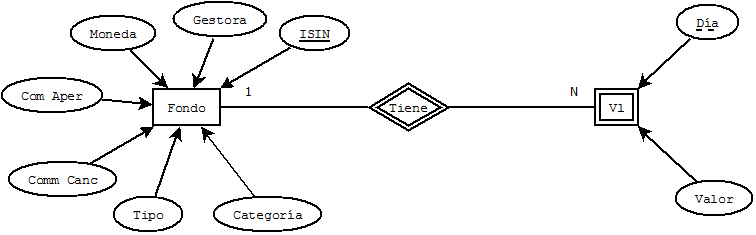
\includegraphics[width=\textwidth]{figuras/ERSimple.png}
	\caption{Diagrama ER inicial.}
	\label{fig:erinicial}
\end {figure}

Este modelo está compuesto por una entidad fuerte encargada de guardar la información referente a los fondos y una débil, que presenta una dependencia de identificación con la primera, encargada de guardar los \gls{VL}s de cada fondo. Por tanto, cada fondo puede tener N \gls{VL}s y cada \gls{VL} sólo puede pertenecer a un fondo.

\newpage

Este modelo permite almacenar los datos básicos tanto de un fondo como el histórico de sus \gls{VL}s, pero no permite realizar operaciones de compra/venta de participaciones. Para poder realizar operaciones sobre los diferentes fondos es necesario añadir un poco de complejidad al modelo:

\begin{figure}[htbp]
	\centering
	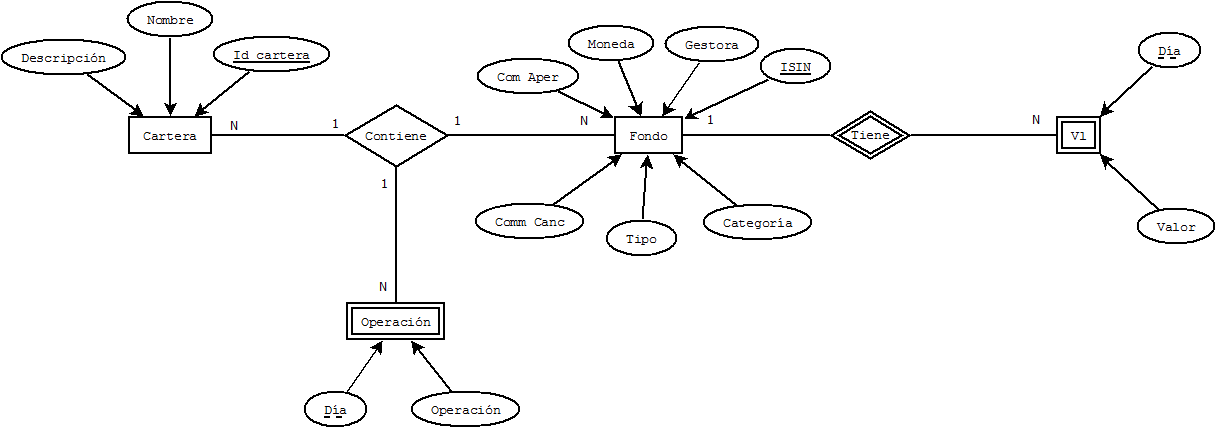
\includegraphics[width=\textwidth]{figuras/ERCompleto.png}
	\caption{Diagrama ER final}
	\label{fig:erfinal}
	\end {figure}

%Diria que esta aproximacion no es correcta, ¿Quizas una entidad debil en el medio en lugar de la relacion "contiene"?


De esta forma incorporamos la posibilidad de tener carteras de fondos y realizar operaciones de compra/venta de participaciones en diferentes fondos pertenecientes a diferentes carteras.\\

Cada fondo de inversión puede pertenecer a varias carteras distintas y cada cartera estará compuesta por varios fondos. Las operaciones sobre ellos sólo estarán permitidas si pertenecen a una cartera de inversión. En caso contrario, sólo se podrá acceder a su histórico de \gls{VL}s.\\

Una vez terminado el diagrama \gls{ER}, el siguiente paso es realizar su conversión al modelo relacional. El resultado es el siguiente:\\

\begin{figure}[htbp]
	\centering
	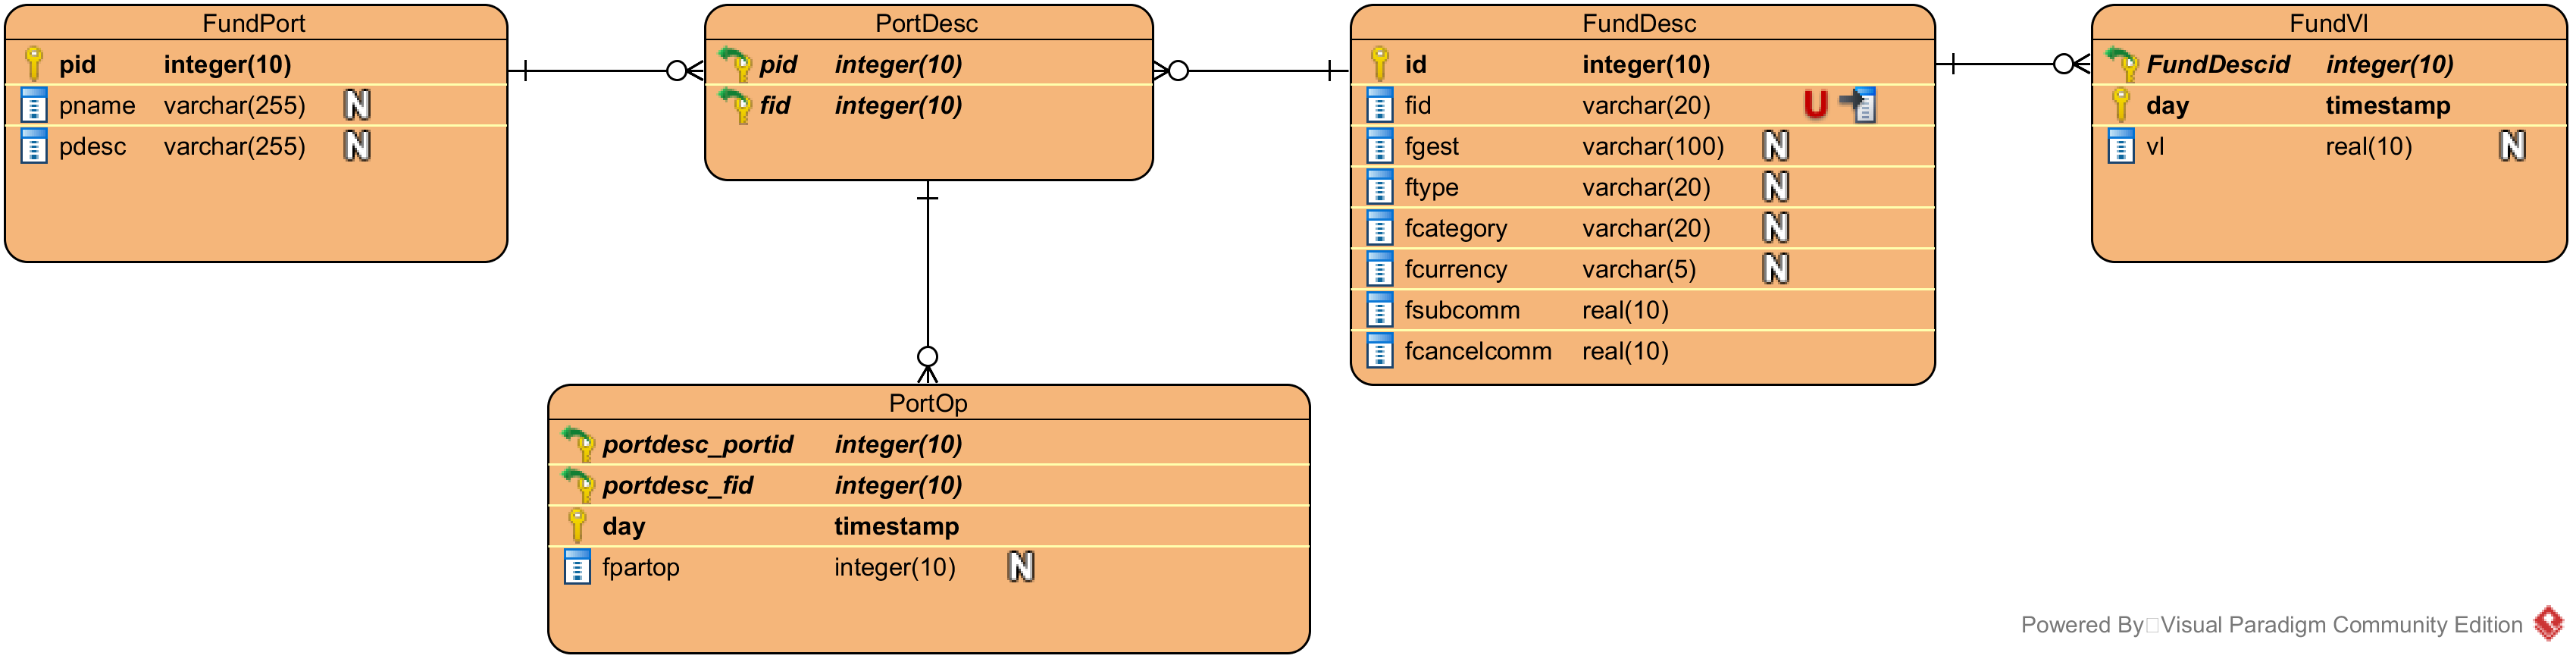
\includegraphics[width=\textwidth]{figuras/DiagramaR.png}
	\caption{Diagrama del modelo relacional (eliminar los nulos)}
	\label{fig:relacional}
	\end {figure}
	
\newpage

\subsection{Implementación de la base de datos mediante Hibernate}

Para implementar la base de datos usando Hibernate, primero debemos modelar las clases Java correspondientes a las tablas del modelo relacional:\\

\begin{figure}[htbp]
	\centering
	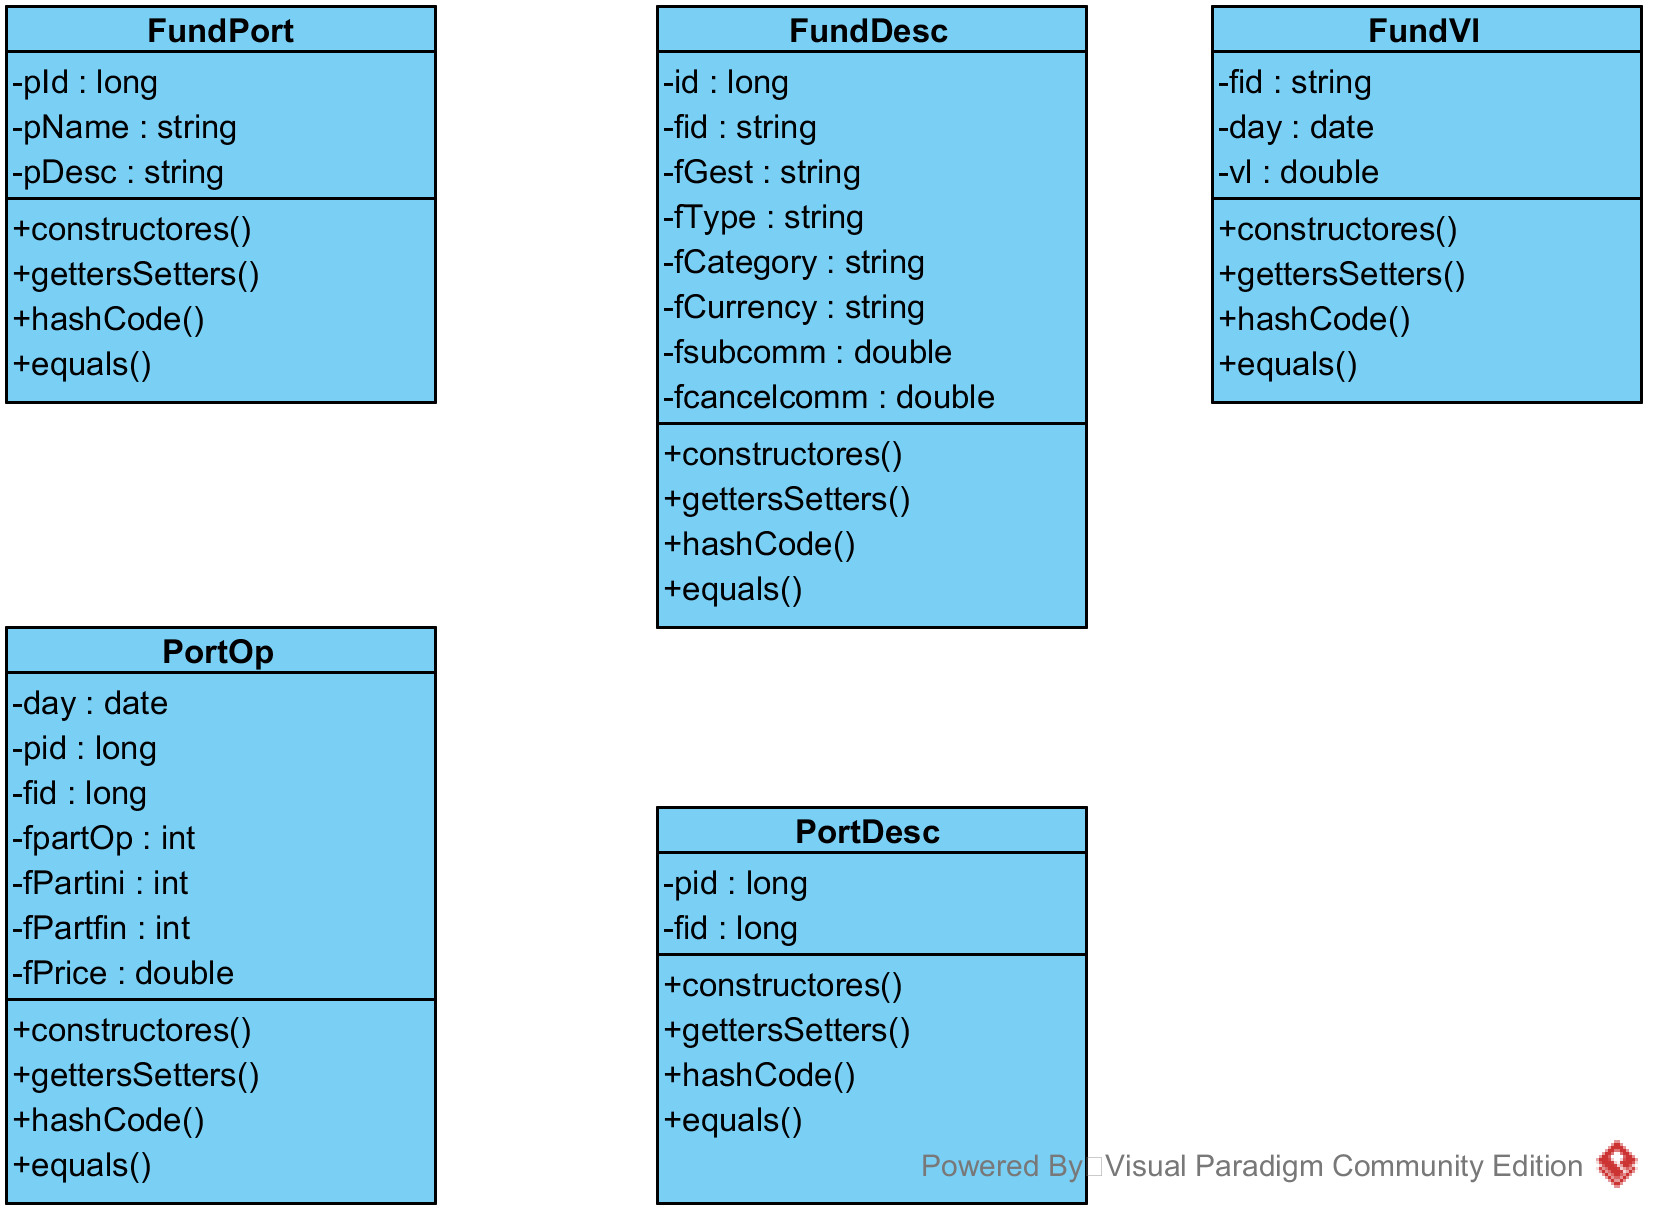
\includegraphics[width=\textwidth]{figuras/Diagrama_clases.png}
	\caption{Diagrama de clases del modelo.}
	\label{fig:mclases}
	\end {figure}

Los atributos de FundDesc, \textbf{id} y de FundPort \textbf{pId}, están formados por valores autogenerados por la base de datos mediante la estrategia de generación \textit{``GenerationType.IDENTITY"} y actúan como claves primarias de las tablas. En el caso de FunDesc el atributo fId (que se corresponde con el \gls{ISIN} del fondo) es una clave candidata que se guardará en la base de datos como un Varchar de longitud 12, indicando a Hibernate que es un valor único y no puede ser nulo. Este atributo podría haberse utilizado como clave primaria de la tabla FundDesc, pero al tratarse de un tipo de dato Varchar que se repetirá, como norma general, más de un millar de veces por cada fondo en la tabla FundVl, se ha decidido utilizar un id autogenerado por motivos de rendimiento.\\

Para que Hibernate mapee las relaciones es necesario incluir en cada una de las clases con relación 1:N una lista con los objetos relacionados. Por ejemplo, cada objeto FunDesc tiene, a mayores de los atributos mostrados en el \gls{UML}, uno llamado fundVls y otro llamado portDescs, que contienen una lista de los FundVls y PortDescs relacionados con ese fondo, respectivamente.\\

\newpage

En el caso de las relaciones N:1 basta con incluir un atributo del tipo del objeto con el que se relaciona. Por ejemplo, cada objeto FundVl tiene un atributo llamado fundDesc que contiene el fondo al que pertenece ese FundVl. Por este motivo, ha sido necesario modificar la implementación por defecto de los métodos equals y hashcode, para que su uso no provocase una llamada recursiva infinita que causase una excepción por stack overflow.\\


Para poder implementar las clases correspondientes a tablas con claves compuestas en Hibernate, es necesario implementar clases serializables que contengan únicamente los atributos que componen la clave primaria de la tabla. En este caso se han implementado las tres necesarias: % Cambiar por uml?

\begin{itemize}
	\item \textbf{FundVlPk:} Con los atributos fundDesc y day.
	\item \textbf{PortDescPk:} Con los atributos funDescId y fundPortId.
	\item \textbf{PortOpPk:} Con los atributos portDesc y day.
\end{itemize}

En el caso de PortOpPk, el atributo portDesc es mapeado en base de datos como el conjunto de las ids del fondo y de la cartera.\\

A continuación, se definen las anotaciones de Hibernate utilizadas para crear la base de datos.

\begin{itemize}
	\item \textbf{@Id:} Indica que el siguiente atributo es la clave primaria de la tabla.
	\item @\textbf{IdClass}: Indica la clase que contiene los atributos que componen la clave primaria de la clase/tabla actual.
	\item  \textbf{@Column:} Indica que el siguiente atributo se modela como una columna en la base de datos.
	\item  \textbf{@Transient:} Indica que el siguiente atributo no se modela como una columna en la base de datos.
	\item \textbf{@GeneratedValue:} Indica que el siguiente atributo es generado automáticamente por la base de datos, utilizando la estrategia asignada.
	\item \textbf{@OneToMany:} Indica que el objeto tiene una relación 1:N con otra tabla.
	\item\textbf{@ManyToOne:} Indica que el objeto tiene una relación N:1 con otra tabla.
	\item\textbf{@JoinColumn:} Indica que el objeto obtiene una columna de otra tabla, normalmente se utiliza junto con la anotación anterior.\\
\end{itemize}

La anotación \textbf{@Transient} se utiliza en la clase PortOp para indicar que los atributos fPartIni, fPartFin y fPrice no se guardan en la base de datos y serán calculados bajo demanda cuando se realice una operación de búsqueda.

\newpage
Las anotaciones @OneToMany y @ManyToOne tienen algunas opciones interesantes:
\begin{itemize}
	\item La opción \textbf{fetch} indica si las listas de objetos relacionados se cargaran bajo demanda (EAGER) o inmediatamente (LAZY).
	\item La opción \textbf{cascade} hace referencia a las acciones que se deben de llevar a cabo tras la eliminación de un objeto, CascadeType.REMOVE indica que se deben eliminar todos los objetos relacionados con él (Por ejemplo, si se elimina un FundDesc se eliminan también todos sus FundVls).
	\item La opción \textbf{mappedBy} se utiliza para definir el atributo que mapea la relación entre las tablas.\\
\end{itemize}

 El último paso para crear la base de datos consiste en indicar a Hibernate cuáles son las clases que debe mapear en su fichero de configuración \textit{``src/main/resources/hibernate.cfg.xml''}.\\
 
  De esta forma, cuando realicemos la llamada de inicio de sesión \textit{``sessionFactory = new Configuration().configure().buildSessionFactory()"} Hibernate generará las tablas en la base de datos, si no existían previamente.\\
 
  La propiedad \textit{``hbm2ddl.auto"} nos permite controlar el comportamiento de hibernate cuando se inicia la sesión. Podemos, desde eliminar las tablas y volver a crearlas en cada inicio, hasta simplemente actualizarlas si hay cambios.

\newpage

\subsection{Implementación del servicio del modelo}

El servicio del modelo será el encargado de exponer las funcionalidades necesarias para el funcionamiento lógico de la aplicación.\\

Como funcionalidades mínimas necesitamos tener la capacidad de añadir, buscar, actualizar y eliminar elementos de cada una de las tablas de la base de datos, pero a la hora de realizar gráficas es muy interesante, por ejemplo, la posibilidad de obtener los \gls{VL}s y las operaciones sobre un fondo en un rango de fechas determinado, por lo que el servicio consta de los siguientes métodos:\\

\begin{figure}[htbp]
	\centering
	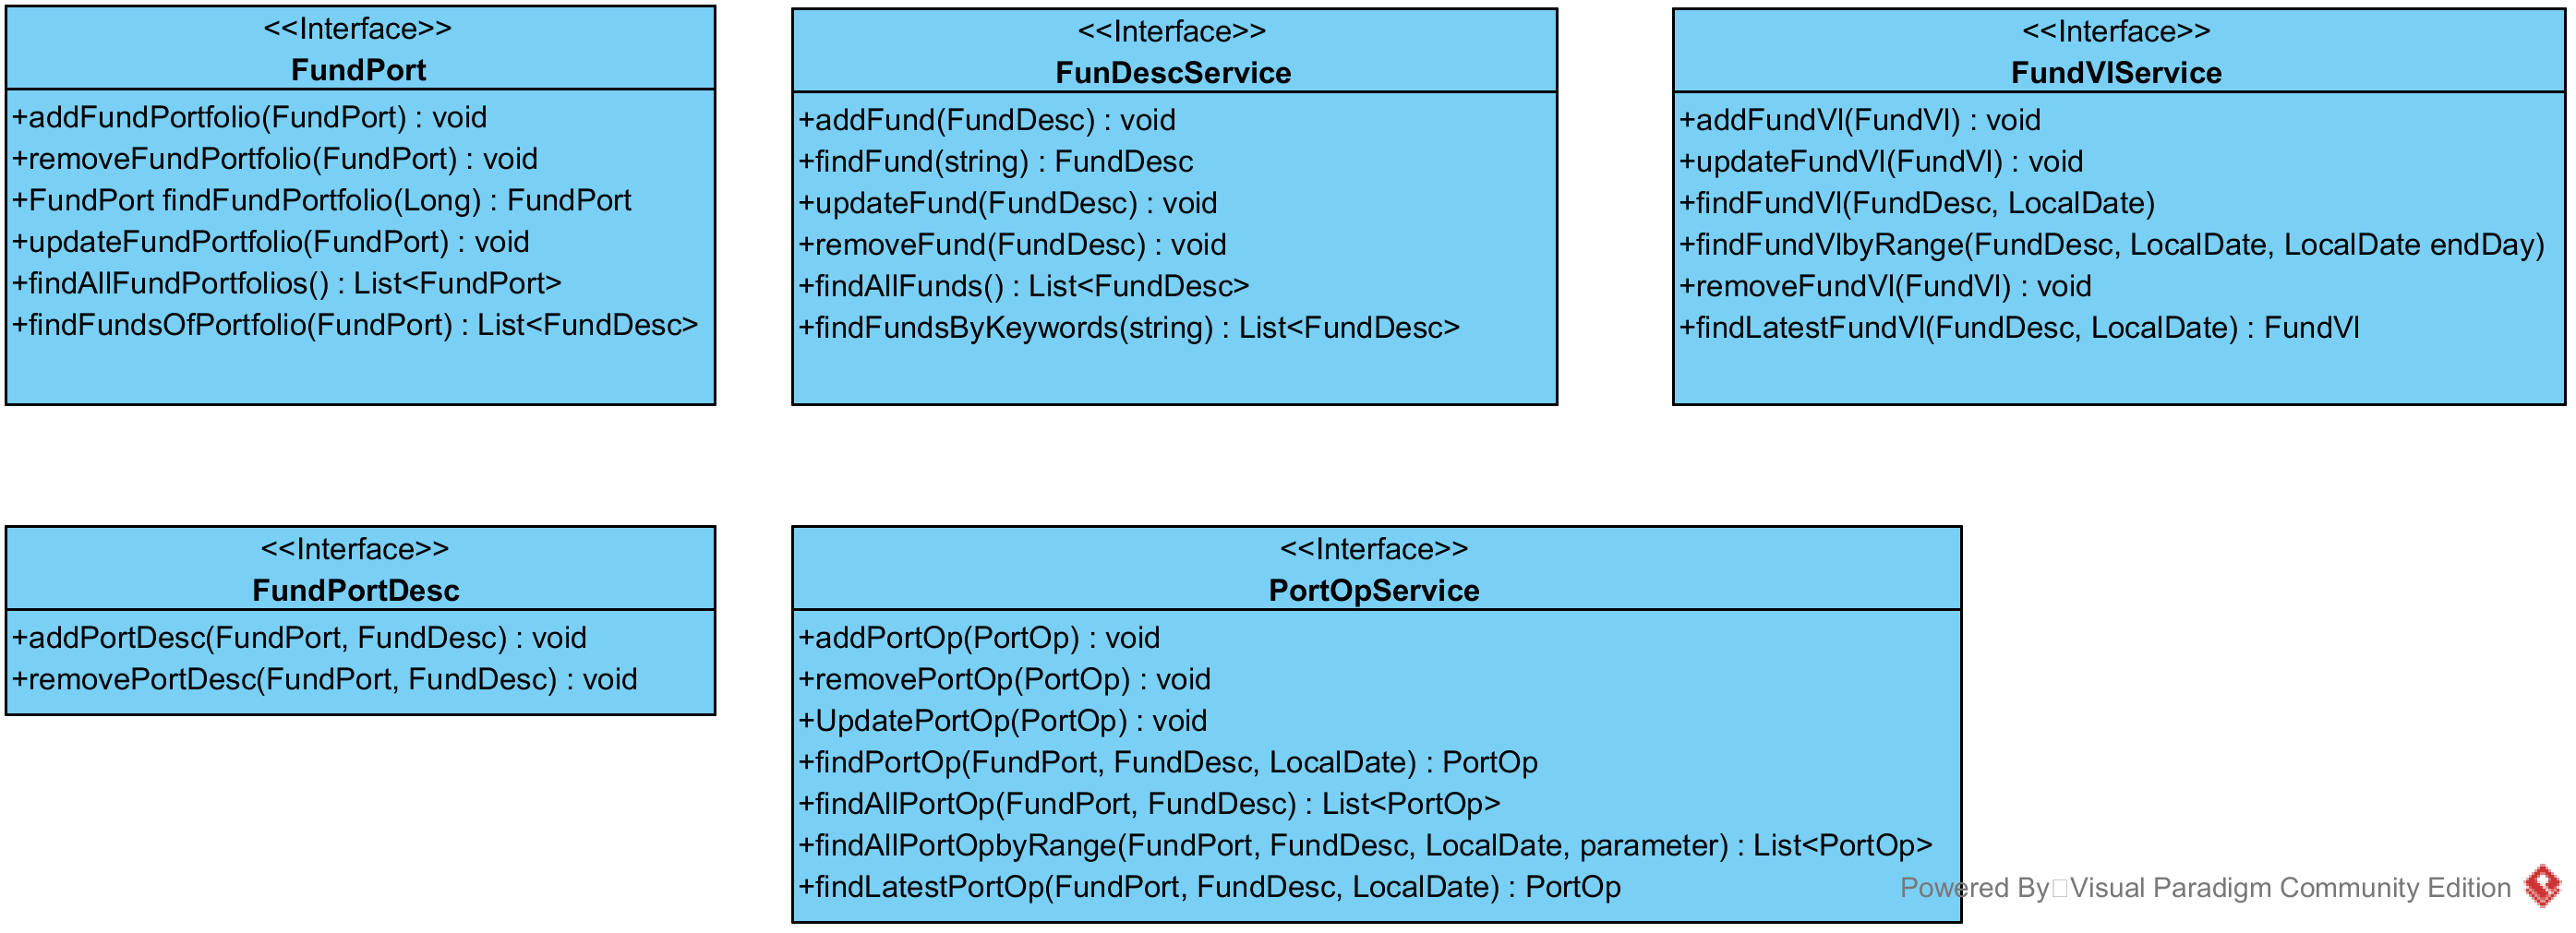
\includegraphics[width=\textwidth]{figuras/Diagrama_Modelo.png}
	\caption{Diagrama del servicio}
	\label{fig:relacional}
	\end {figure}

Aunque en este diagrama existe una interfaz del servicio para cada clase, en la implementación se han agrupado todos en una única interfaz denominada \textbf{FundService}.\\

Cada uno de los métodos del servicio lanza una \textbf{RunTimeException} si se produce algun error a la hora de conectarse a la base de datos. A mayores, se han implementado dos excepciones más:

\begin{itemize}
	\item \textbf{InputValidationException:} Se produce cuando los datos introducidos por el usuario no son correctos.
	\item \textbf{InstanceNotFoundException:} Se produce cuando no se puede encontrar el objeto solicitado en la base de datos.
\end{itemize}


Para llevar a cabo la validación de los datos de entrada se ha incorporado un validador: \\

uml del validador\\

\newpage

Existen una serie de métodos en el servicio que utilizan este validador para asegurar que los datos introducidos son correctos:

\begin{itemize}
	\item \textbf{validateFundVl:} Se encarga de validar si el campo \gls{VL} del FundVl es mayor o igual que cero.
	\item \textbf{validateFund:} Se encarga de validar que el \gls{ISIN} del fondo es correcto y llama a su vez a validateFundVl para validar cada uno de sus FundVl.
	\item \textbf{validateFundPort:} Se encarga de validar que el nombre de la cartera de fondos no sea un string vacío.
	\item \textbf{validatePortOp:} Se encarga de validar que la operación añadida, eliminada o actualizada no deje en ningún momento a la base de datos con un total de participaciones negativo.
\end{itemize}

Ahora analizaremos cada método por separado:

\begin{itemize}
	\item FundDesc
						 \begin{itemize}
							\item \textbf{addFund:} añade un FundDesc y toda su lista de FundVLs a la base de datos. La forma más común de representación de un fondo es mediante un fichero excel (.xls) que contenga un conjunto de pares día-\gls{VL}, en un futuro la aplicación permitirá importar los \gls{VL}s a partir de estos ficheros, por lo que se podrán guardar en la base de datos simplemente llamando a esta operación.
							\item \textbf{findFund:} devuelve el FundDesc a partir de su \gls{ISIN}. A pesar de que la clave primaria de la tabla sea la clave subrogada \textit{``id"}, es más natural buscar un fondo en concreto por su \gls{ISIN}.
							\item \textbf{updateFund:} actualiza los campos de un FundDesc.
							\item \textbf{removeFund:} elimina un FundDesc y toda su lista de FundVls de la base de datos.
							\item \textbf{findAllFunds:} obtiene todos los FundDesc de la base de datos.
							\item \textbf{findFundsByKeywords:} obtiene los fundDesc que coinciden con una serie de caracteres en alguno de sus campos. Esta función es útil a la hora de buscar varios fondos de un mismo tipo, moneda o gestora, por ejemplo.
				 		 \end{itemize}
	\item FundPort
						\begin{itemize}
							\item \textbf{addFundPortfolio:} añade una cartera de fondos.
							\item \textbf{removeFundPortfolio:} elimina una cartera de fondos.
							\item \textbf{findFundPortfolio:} obtiene una cartera de fondos a partir de su Id.
							\item \textbf{updateFundPortfolio:} actualiza los campos de una cartera de fondos.
							\item \textbf{findAllFundPortfolios:} obtiene todas las carteras de la base de datos.
							\item \textbf{findFundsOfPortfolio:} obtiene todos los fondos de una cartera.
						\end{itemize}
					\newpage
	\item FundVl
						\begin{itemize}
							\item\textbf{addFundVl:} añade un unico FundVl a un fondo en un día concreto.
							\item\textbf{removeFundVl:} elimina una fila de la tabla \gls{VL} de un fondo en un día concreto.
							\item \textbf{findFundVl:} obtiene el FundVl de un fondo en un día concreto.
							\item \textbf{updateFundVl:} actualiza un único FundVl de un fondo en un día concreto.
							\item \textbf{findFundVlByRange:} obtiene los Vl de un fondo dado en el intervalo de tiempo deseado.
							\item \textbf{findLatestFundVl:} obtiene el FundVl del día mas próximo a uno dado (se comporta exactamente igual a findFundVl si existe un valor vl en ese día). Esta función se utiliza para calcular el valor monetario de una operación. Cuando no se disponga del \gls{VL} de un fondo el día de la operación, se utilizará en su lugar el valor del día anterior más cercano.
						\end{itemize}
				
	\item PortDesc
						\begin{itemize}
							\item\textbf{addPortDesc:} añade un fondo a una cartera.
							\item\textbf{removePortDesc:} elimina un fondo de una cartera.
						\end{itemize}
	\item PortOp
						\begin{itemize}
							\item\textbf{addPortOp:} añade una operación (con participaciones como unidad) sobre un fondo en una cartera en un día determinado.
							\item\textbf{removePortOp:} elimina una operación realizada sobre un fondo en una cartera en una fecha.
							\item \textbf{findPortOp:} obtiene una operación sobre un fondo en una cartera en un día determinado.
							\item \textbf{updatePortOp:} actualiza un PortOp (con participaciones como unidad) sobre un fondo en una cartera en un día determinado.
							\item \textbf{findAllPortOp:} devuelve todas las operaciones realizadas sobre un fondo en una cartera.
							\item \textbf{findPortOpByRange:} devuelve todas las operaciones realizadas sobre un fondo en una cartera entre dos fechas.
							\item \textbf{findLatestPortOp:} obtiene la operación sobre un fondo en una cartera del día mas próximo a un día dado (Se comporta exactamente igual a findPortOp si existe un PortOp en ese día). Esta función se utiliza para conocer cual ha sido la operación más reciente sobre un fondo, lo que permite ver las participaciones que tenemos invertidas en él.\\
						\end{itemize}
	
\end{itemize}

Como se ha comentado anteriormente, los campos de los objetos PortOp:  fPartIni, fPartFin y fPrice, se calculan bajo demanda en los métodos de búsqueda findPortOp, findAllPortOp, findPortOpByRange y findLatestPortOp. La operación encargada de calcularlos es calculatePortOp.\\

\newpage

El método \textbf{calculatePortOp} revisa todas las operaciones anteriores y obtiene el numero de participaciones inicial y final, además del precio de la operación, utilizando para ello el \gls{VL} más próximo y teniendo en cuenta las comisiones de apertura y cancelación del fondo.\\

Se utiliza esta operación en lugar de almacenar directamente los valores de los campos en la base de datos debido a que si se guardasen, cada inserción, actualización o borrado de una operación, implicaría actualizar todos los valores de las operaciones siguientes, además de estar guardando información redundante que se puede calcular directamente con los datos que ya se encuentran en la base de datos.



\newpage
\section{Segunda iteración: Creación de la GUI}

Esta segunda iteración del desarrollo tiene como objetivo construir la \gls{GUI}, que será la encargada tanto de mostrar los datos al usuario como de proveer de datos al modelo.
\\

La biblioteca gráfica utilizada es Swing, un framework MVC para desarrollar interfaces gráficas para Java con independencia de la plataforma.

\subsection{Diseño de la interfaz}

Como en el apartado anterior, para comenzar a diseñar la interfaz debemos tener en cuenta la estructura de datos que tenemos, las funcionalidades del modelo que queremos exponer, y la forma en que el usuario interactuará con ellas.
\\

Nuestro modelo de carteras con fondos se asemeja mucho a una estructura de árbol, las carteras serían los nodos padre mientras que cada fondo sería una hoja conectado con una o varias carteras. imagen del árbol genérico.
\\

De esta forma con un simple vistazo podemos ver la distribución de los diferentes fondos de la aplicación.
\\

Para que la interacción con la aplicación por parte del usuario sea más sencilla, de cada nodo del árbol emergerá un menú con las diferentes opciones de cada elemento, dependiendo de si es un fondo o una cartera:

\begin{itemize}
	\item \textbf{Fondo:}
	\begin{itemize}
		\item \textbf{Añadir Vl:} muestra un dialogo para añadir un \gls{VL} al fondo.
		\item \textbf{Actualizar:} muestra un dialogo para actualizar los campos del fondo.
		\item \textbf{Borrar:} elimina el fondo de la base de datos.
		\item \textbf{Ver Vls:} muestra una tabla con los \gls{VL}s del fondo.
		\item \textbf{Importar Vls:} permite importar un conjunto de \gls{VL}s de un fichero .xls si este tiene el formato correcto.
		\item \textbf{Exportar Fondo:} exporta el fondo a un fichero .xls en el directorio seleccionado.
	\end{itemize}
\end{itemize}
\newpage
\begin{itemize}
	\item \textbf{Cartera}:
	\begin{itemize}
		\item\textbf{Añadir fondo:} muestra un dialogo para añadir un fondo a la cartera.
		\item \textbf{Eliminar fondo:} muestra un dialogo para eliminar un fondo de una cartera.
		\item \textbf{Actualizar cartera:} muestra un dialogo para actualizar los campos de una cartera.
		\item \textbf{Borrar cartera}: elimina la cartera de la base de datos.
		\item \textbf{Añadir operación:} muestra un dialogo para añadir una operación a la cartera sobre un fondo determinado.
		\item \textbf{Ver operaciones:} muestra una tabla con las operaciones de la cartera sobre un fondo determinado.\\
	\end{itemize}
\end{itemize}

Las funcionalidades que no se encuentran en los anteriores menús estarán disponibles en el menú principal de la aplicación.

\begin{itemize}
	\item \textbf{Archivo}:
	\begin{itemize}
		\item\textbf{Añadir fondo:} muestra un dialogo para añadir un fondo a la base de datos.
		\item \textbf{Añadir cartera:} muestra un dialogo para añadir una cartera a la base de datos.
		\item \textbf{Importar fondo:} permite importar un fondo (previamente exportado por la aplicación) de un fichero .xls.\\
	\end{itemize}
\end{itemize}

Para poder representar correctamente las gráficas necesitaremos algunos elementos adicionales: 
\begin{itemize}
	\item Un \textbf{panel} en el que representar las gráficas.
	\item Un \textbf{desplegable} donde seleccionar la gráfica deseada.
	\item Un \textbf{campo de texto} donde incluir una pequeña descripción de lo que representa cada gráfica.
	\item Para las gráficas en las que necesitemos seleccionar un intervalo de tiempo determinado, debemos incluir \textbf{dos calendarios} que nos permitan acotar las fechas de inicio y fin del intervalo.
	\item Para la gráfica de la rentabilidad estimada, necesitamos un pequeño \textbf{campo de entrada} donde poder introducir una rentabilidad por si el usuario no quiere usar la del fondo.
	\item Para la gráfica de medias móviles, necesitaremos \textbf{botones} para seleccionar los intervalos de tiempo.
\end{itemize}


Una primera aproximación de la interfaz principal constará del árbol de las carteras, una barra de menú principal y los elementos necesarios para representar las gráficas.

\newpage

\subsection{Implementación de la interfaz}

Con las necesidades de diseño que hemos establecido en el punto anterior, el siguiente paso es seleccionar los componentes para crear la interfaz en Swing.
\\

Comenzamos por implementar la ventana principal de la aplicación, para ello, Swing nos proporciona la clase \textbf{JFrame}. Un \textbf{JFrame} es una ventana de alto nivel sobre la que podemos añadir el resto de componentes de la interfaz de manera sencilla.
\\

Los primeros elementos que añadiremos serán la barra del menú (\textbf{JMenuBar} en Swing), que se ajusta automáticamente a la parte superior de la ventana, y el panel para las gráficas (\textbf{JPanel} en Swing).
\\

Los componentes en Swing se alinean unos con otros mediante ``\textit{gaps}". Estos espacios pueden ser de tamaño fijo (se respeta su tamaño aunque se redimensione la interfaz) o de tamaño variable (se expanden o se contraen si se redimensiona la interfaz).

\begin{figure}[htbp]
	\centering
	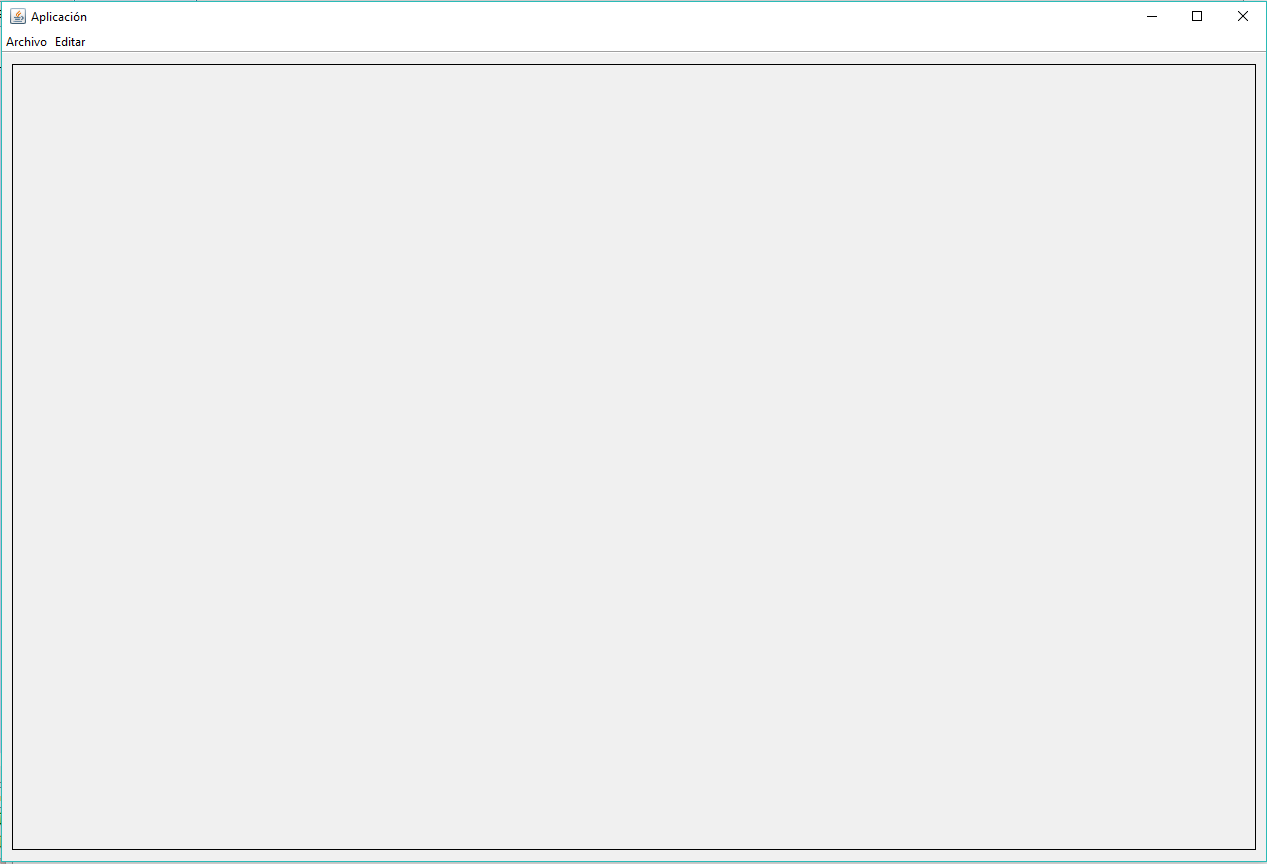
\includegraphics[width=\textwidth]{figuras/gui1.PNG}
	\caption{JFrame}
	\label{fig:gui1}
	\end {figure}


\newpage


Una vez creada la ventana principal, el siguiente paso es añadir el árbol para representar las carteras y los fondos. Swing nos proporciona esta estructura en la clase  \href{JTree}{\textbf{JTree}}, mediante la cual podemos crear un árbol con la estructura de datos deseada.\\


\begin{figure}[htbp]
	\centering
	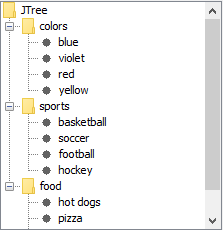
\includegraphics[width=5cm]{figuras/JTree.PNG}
	\caption{JTree}
	\label{fig:JTree}
	\end {figure}

Como se puede observar en la figura anterior, cada uno de los nodos padre se puede expandir o contraer a voluntad del usuario. Por ello es obligatorio incluir el árbol en un contenedor que permita el desplazamiento vertical. En Swing contamos con la clase \textbf{JScrollPane} que nos permite realizar esta función.
\\

El desplegable para seleccionar las gráficas se implementa mediante un \textbf{JComboBox}, de tal forma que el nombre de cada gráfica será un elemento de dicho desplegable. Cada componente de Swing nos permite añadirle \textit{``action listeners"} que se encargan de capturar los eventos que van sucediendo, por ejemplo, la selección de un elemento del desplegable o del árbol, permitiéndonos reaccionar ante ellos de la forma adecuada.

\begin{figure}[htbp]
	\centering
	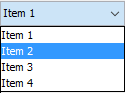
\includegraphics{figuras/JComboBox.png}
	\caption{JComboBox}
	\label{fig:JComboBox}
	\end {figure}

Para el campo de texto de descripción de las gráficas se utiliza un \textbf{JEditorPane}, que nos proporciona un recuadro para mostrar texto formateado. Como en el caso anterior, es necesario incluir este componente en un JScrollPane.

\begin{figure}[htbp]
	\centering
	
\includegraphics{figuras/JEditorPane.png}
	\caption{JEditorPane}
	\label{fig:JEditorPane}
	\end {figure}
\newpage

El siguiente paso es añadir a la interfaz los elementos adicionales que necesitan las gráficas.\\

Para los calendarios de las fechas de inicio y fin de intervalo utilizamos el componente \textbf{JDatePanel}, que nos proporciona un calendario en el que el usuario puede seleccionar una fecha. En nuestra aplicación se utiliza la clase \textit{``LocalDate"} para los datos de tipo fecha, por lo tanto para que los calendarios nos muestren las fechas en el formato correcto es necesario crear una clase que redefina los métodos \textit{``stringToValue"} y \textit{``valueToString"} de la clase \textit{``AbstractFormatter"} con el formato utilizado por LocalDate: \textit{``yyyy-MM-dd"}.

\begin{figure}[htbp]
	\centering
	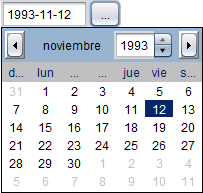
\includegraphics[width=5cm]{figuras/JDatePanel.png}
	\caption{JDatePanel}
	\label{fig:JDatePanel}
	\end {figure}

Los botones de selección de período, utilizados para calcular las medias móviles, están formados por tres \textbf{JRadioButton} incluidos en un \textbf{ButtonGroup}. De esta manera solo se podrá seleccionar uno de los tres botones a la vez.

\begin{figure}[htbp]
	\centering
	
\includegraphics{figuras/ButtonGroup.png}
	\caption{ButtonGroup}
	\label{fig:ButtonGroup}
	\end {figure}
	
Para poder introducir una rentabilidad estimada, se utilizan en conjunto una \textbf{JLabel} un \textbf{JFormattedTextField} y un \textbf{JButton}. La etiqueta contiene la descripción del parámetro que se debe introducir en el campo de texto y el botón simplemente llevará a cabo los cálculos.

\begin{figure}[htbp]
	\centering
	\includegraphics{figuras/Calculos.png}
	\caption{Rentabilidad estimada}
	\label{fig:calculos}
	\end {figure}

La entrada de texto acepta entradas de números reales con dos decimales, si se introduce texto, por ejemplo, el campo lo descarta y toma el último valor válido.
\newpage

Con todos estos elementos añadidos la interfaz queda de la siguiente manera:

\begin{figure}[htbp]
	\centering
	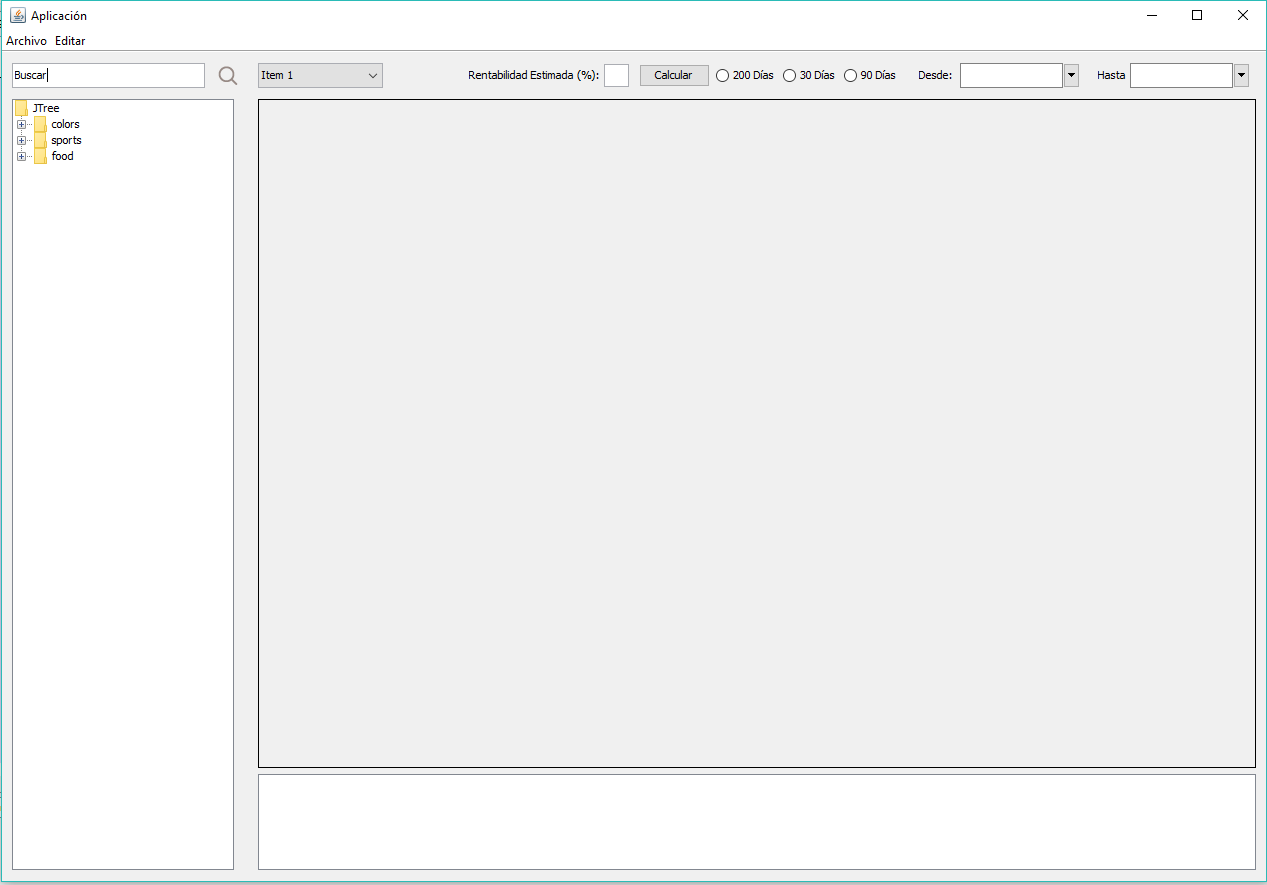
\includegraphics[width=\textwidth]{figuras/gui2.PNG}
	\caption{GUI}
	\label{fig:gui2}
	\end {figure}

Swing nos permite ocultar y mostrar componentes de la interfaz bajo demanda. Dependiendo de la gráfica seleccionada las fechas, los botones o el recuadro de introducir la rentabilidad esperada se ocultarán. Los restantes elementos visibles se alinearan siempre a la derecha.\\
\newpage

El árbol, una vez actualizado, es el contenedor de los datos de carteras y de fondos. Como se había establecido, cuando hagamos click derecho en una de las carteras o fondos, se nos mostrará un menú emergente (\textbf{JPopupMenu} en Swing) con los elementos seleccionados en el diseño (\textbf{JMenuItem} en Swing):

	
	\begin{figure}[htbp]
		\centering
		\subfigure[Cartera]{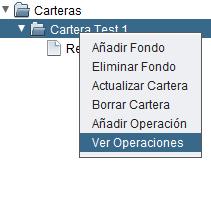
\includegraphics{figuras/menucartera.PNG}}
		\subfigure[Fondo]{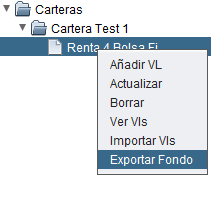
\includegraphics{figuras/menufondo.PNG}}
		\caption{Popup menú} \label{fig:menucartera}
	\end{figure}

Cada elemento del popup menú crea una ventana emergente que muestra lo siguiente:

\begin{itemize}
	\item \textbf{Fondo:}
	\begin{itemize}
		\item \textbf{Añadir Vl :} muestra un dialogo compuesto por varias etiquetas indicando los nombres de  los campos de entrada, un calendario para seleccionar la fecha del \gls{VL}, un campo de texto formateado para indicar el valor y dos botones para aceptar o cancelar la operación. Si al aceptar, la operación no se puede realizar, se muestra una ventana de error.
		\item \textbf{Actualizar:} muestra un dialogo compuesto por varias etiquetas, una para cada atrubuto de la clase FundDesc, y entradas de texto con los valores actuales del fondo, de esta manera el usuario puede sobrescribir cualquier campo viendo el valor que posee actualmente el fondo. 
		\item \textbf{Borrar:} muestra un dialogo de confirmación con las opciones si o no.
		\item \textbf{Ver Vls:} muestra un dialogo con una tabla que contiene todos los \gls{VL}s del fondo seleccionado.
		\item \textbf{Importar Vls:} muestra un dialogo de selección del fichero de origen. Si el fichero no tiene un formato válido se muestra una ventana de error.
		\item \textbf{Exportar Fondo:} muestra un dialogo de selección del fichero de destino.
	\end{itemize}
\end{itemize}
\newpage
\begin{itemize}
	\item \textbf{Cartera}:
	\begin{itemize}
		\item\textbf{Añadir fondo:} muestra un dialogo compuesto por una etiqueta indicando la cartera seleccionada, un desplegable con los fondos que todavía no han sido añadidos a la cartera y dos botones para aceptar o cancelar la operación.
		\item \textbf{Eliminar fondo:} muestra un dialogo compuesto por una etiqueta indicando la cartera seleccionada, un desplegable con los fondos que han sido añadidos a la cartera y dos botones para aceptar o cancelar la operación.
		\item \textbf{Actualizar cartera:} muestra un dialogo compuesto por dos etiquetas indicando los nombres de  los campos de entrada y entradas de texto con los valores actuales del nombre y la descripción de la cartera. Si al aceptar, la operación no se puede realizar, se muestra una ventana de error.
		\item \textbf{Borrar cartera}: muestra un dialogo de confirmación con las opciones si o no.
		\item \textbf{Añadir operación:} muestra un dialogo compuesto por varias etiquetas indicando los nombres de  los campos de entrada, un desplegable para seleccionar el fondo, un calendario para seleccionar la fecha de la operación, un campo de texto formateado para indicar el total de participaciones de la operación, dos botones para seleccionar si la operación es de compra o de venta y otros dos botones para aceptar o cancelar la operación. Si al aceptar, la operación no se puede realizar, se muestra una ventana de error.
		\item \textbf{Ver operaciones:} muestra un dialogo con una tabla que contiene todas las operaciones del fondo seleccionado.\\
	\end{itemize}
\end{itemize}

Todos los métodos que abren un dialogo con el usuario utilizan la clase \textbf{JDialog} como ventana emergente, excepto las ventanas de error y las de selección de fichero.\\

Las ventanas de error y de confirmación de borrado se crean utilizando la clase \textbf{JOptionPane}, que nos proporciona una manera fácil y rápida de proveer al usuario de información, así como de solicitar confirmación. \\

	\begin{figure}[htbp]
	\centering
	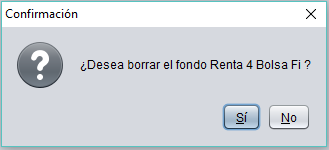
\includegraphics{figuras/confirmacion.PNG}
	\caption{Ventana de confirmación}
	\label{fig:confirmacion}
	\end {figure}
\newpage

La selección de ficheros se implementa usando la clase \textbf{JFileChooser} que nos provee de un pequeño explorador de archivos para seleccionar la ruta del fichero a importar o exportar. Es posible personalizar el tipo de archivos que admite o seleccionar un nombre y extensión predeterminados a la hora de exportar los fondos.

	\begin{figure}[htbp]
	\centering
	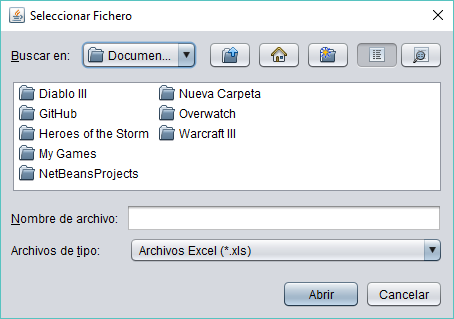
\includegraphics{figuras/fichero.PNG}
	\caption{Ventana de selección de fichero}
	\label{fig:fichero}
	\end {figure}

La tabla de \gls{VL}s esta implementada mediante la clase \textbf{JTable} en un contenedor de tipo JScrollPanel.

	\begin{figure}[htbp]
	\centering
	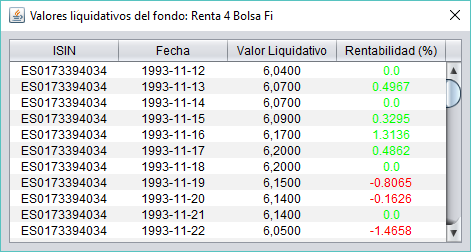
\includegraphics[width=12cm]{figuras/vls.PNG}
	\caption{Tabla de valores liquidativos}
	\label{fig:vls}
	\end {figure}
	
Como se puede observar en la figura anterior, la columna de rentabilidad muestra un color distinto en función de su valor, para conseguir este efecto ha sido necesario sobrescribir el método \textit{``prepareRenderer"} de la tabla, de tal forma que si el valor de la columna es negativo se muestre rojo y si es positivo verde.\\
\newpage

Si seleccionamos un día concreto de la tabla y hacemos click derecho sobre él, se muestra un nuevo menú emergente que nos proporciona la posibilidad de actualizar o de borrar el \gls{VL}. El dialogo de actualización es muy similar al de añadir un nuevo \gls{VL} con la diferencia de que el día no puede ser modificado. Si se selecciona la operación de borrado se muestra el menú de confirmación. 
\\

La tabla de operaciones es similar a la de los \gls{VL}s:

	\begin{figure}[htbp]
	\centering
	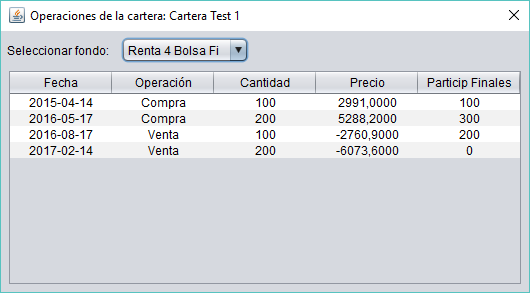
\includegraphics[width=12cm]{figuras/ops.PNG}
	\caption{Tabla de operaciones}
	\label{fig:ops}
	\end {figure}

En ella se muestran todas las operaciones de la cartera para el fondo seleccionado en el desplegable. Como en el caso anterior, si seleccionamos una fila de la tabla, y hacemos click derecho sobre ella, se muestra un nuevo menú emergente que nos proporciona la posibilidad de actualizar o de borrar la operación.
\\

Por último, el menú de archivo contiene las operaciones de añadir un fondo o una cartera e importar un fondo. Los dos primeros muestran un dialogo muy similar a sus versiones de actualizar y el último muestra el selector de ficheros. Todos ellos muestran la ventana de error si no se puede completar la operación.
\newpage

\section{Tercera iteración: Creación de las gráficas}

Esta tercera iteración tiene como objetivo crear el conjunto de gráficas que proveerán de información al usuario acerca de los fondos y las carteras.\\

La lbrería de gráficas utilizada es JFreeChart, un marco de software open source para el lenguaje de programación Java, el cual permite la creación de gráficos complejos de forma simple.

\subsection{Preparación de las gráficas}

El primer paso antes de comenzar a programar las gráficas es decidir donde se van a implementar. En nuestro caso se implementan en una clase aparte llamada \textit{``ChartMaker"}. Esta clase será la encargada de recibir los datos necesarios de la interfaz, crear la gráfica seleccionada y su descripción a partir de ellos y devolverlas a la interfaz para que esta pueda representarlas en el panel.\\

Para pasar la gráfica y la descripción al controlador, se ha creado una clase sencilla denominada \textit{``Chart"}. Esta clase está compuesta por dos atributos, un ChartPanel que será el contenedor y un String con la descripción de la gráfica.\\

JFreeChart funciona de la siguiente manera: primero debemos crear un \textit{``dataset"} acorde con el tipo de gráfica que queramos realizar, por ejemplo, para gráficas en forma de tarta se utiliza \textit{``DefaultPieDataset"} y para gráficas de barras \textit{``DefaultCategoryDataset"}.\\

A continuación, se insertan los datos en el dataset, normalmente mediante el método \textit{``dataset.addValue()"} o \textit{``dataset.setValue()"}. Estos métodos utilizan parámetros distintos dependiendo del tipo de dataset, por ejemplo para las gráficas en forma de tarta se le pasan los siguentes campos.

\begin{verbatim}
pie_chart_dataset.setValue(nombre, valor);
\end{verbatim}

Una vez añadidos todos los valores se invoca a \textit{``ChartFactory"}, en este caso: 

\begin{verbatim}
JFreeChart chart = ChartFactory.createPieChart(nombre de la gráfica,
pie_chart_dataset, leyenda, herramientas, urls);
\end{verbatim}

Donde los campos leyenda, herramientas y urls son de tipo booleano para indicar si se deben incluir dichos elementos el la gráfica.\\

La llamada a \textit{``ChartFactory"} nos devuelve la gráfica creada, ahora solamente necesitamos crear un nuevo ChartPanel con la gráfica y añadirlo al panel de la interfaz.

\begin{verbatim}
ChartPanel cP = new ChartPanel(chart);
panelGraficas.add(cp);
\end{verbatim}
\newpage

\subsection{Gráficas de carteras}

\subsubsection{Distribución de capital de la cartera}

Esta primera gráfica tiene como objetivo, que el usuario pueda ver la distribución del capital invertido en los diferentes fondos de una cartera. Para ello se utiliza una gráfica en forma de tarta en la cual cada una de sus porciones representa el tanto por ciento del capital de la cartera que está invertido en un fondo.\\

	\begin{figure}[htbp]
	\centering
	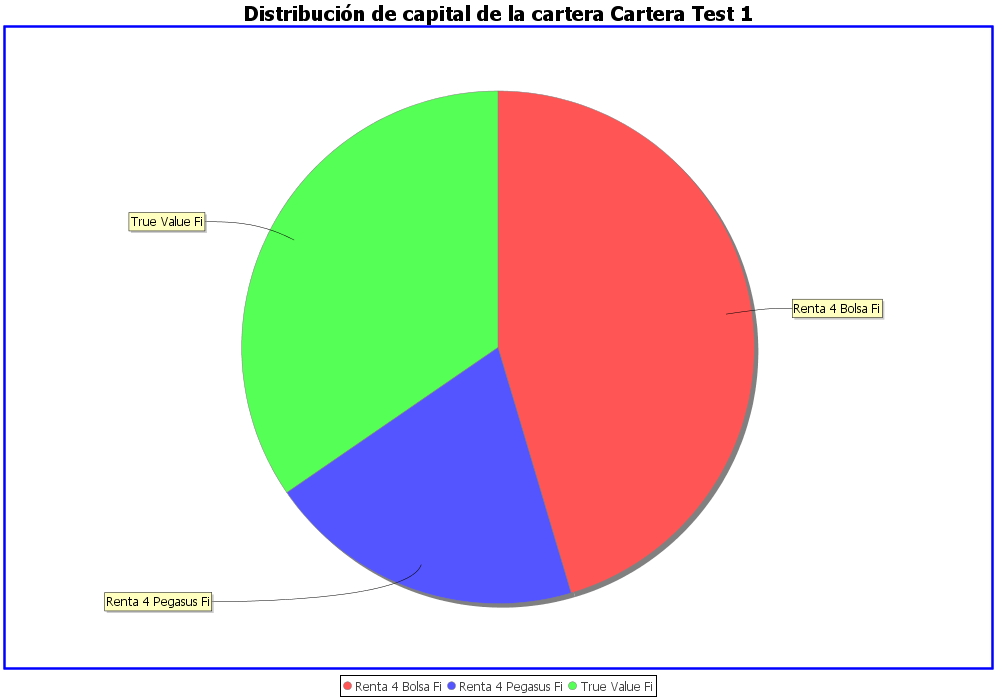
\includegraphics[width=\textwidth]{figuras/distribucion.PNG}
	\caption{Gráfica de distribución de capital de la cartera}
	\label{fig:distribucion}
	\end {figure}
	
Para el cálculo de está gráfica se toma el valor del número de participaciones de cada fondo y se multiplica por el valor de cada una a día de hoy, si no existe un \gls{VL} en el día de hoy se utiliza el más próximo.\\
\newpage

\subsubsection{Fondos normalizados de la cartera}

Esta gráfica tiene como objetivo mostrar un histórico de los \gls{VL}s de todos los fondos de la cartera partiendo todos de la misma base, en este caso 100. De esta manera es posible comparar los fondos entre ellos y ver cuales han alcanzado una mayor rentabilidad. Para ello se utiliza una gráfica de serie temporal. Este tipo de gráficas utilizan valores de tipo temporal en el eje de abscisas y valores de tipo double en el de ordenadas.\\

	\begin{figure}[htbp]
	\centering
	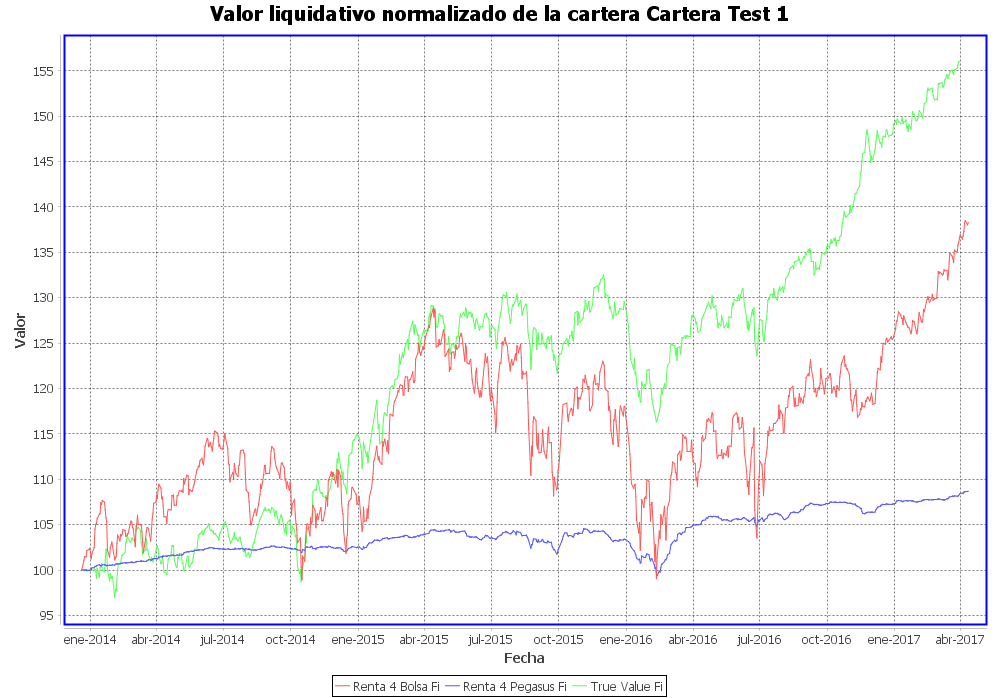
\includegraphics[width=\textwidth]{figuras/normalizados.PNG}
	\caption{Gráfica de fondos normalizados de la cartera}
	\label{fig:normalizados}
	\end {figure}
	
	


Para el cálculo de está gráfica supongamos que el fondo tiene los siguientes valores liquidativos $\text{VL}_1,\text{VL}_2,\ldots,\text{VL}_d$ para los días $1,2,\ldots,d$, y que queremos calcular sus \gls{VL}s normalizados $\text{VLN}_1,\text{VLN}_2,\ldots,\text{VLN}_d$ para que comiencen en 100 . Los valores se calculan de la siguiente manera.

\begin{equation}
\text{VLN}_i=\text{VL}_i\left(\frac{100}{\text{VL}_1}\right)
\end{equation}

	\newpage

\subsubsection{Fondos más y menos rentables de la cartera}

Esta gráfica tiene como objetivo mostrar los cinco fondos más y menos rentables de una cartera. De esta manera es posible ver los mejores y los peores fondos de la cartera y tomar decisiones acerca del capital invertido en ellos, como por ejemplo, sacar fondos del peor y comprar participaciones del mejor con ellos. \\

Para visualizar los datos se utiliza una gráfica de barras donde cada barra corresponde a la rentabilidad del fondo en la cartera.\\


	\begin{figure}[htbp]
	\centering
	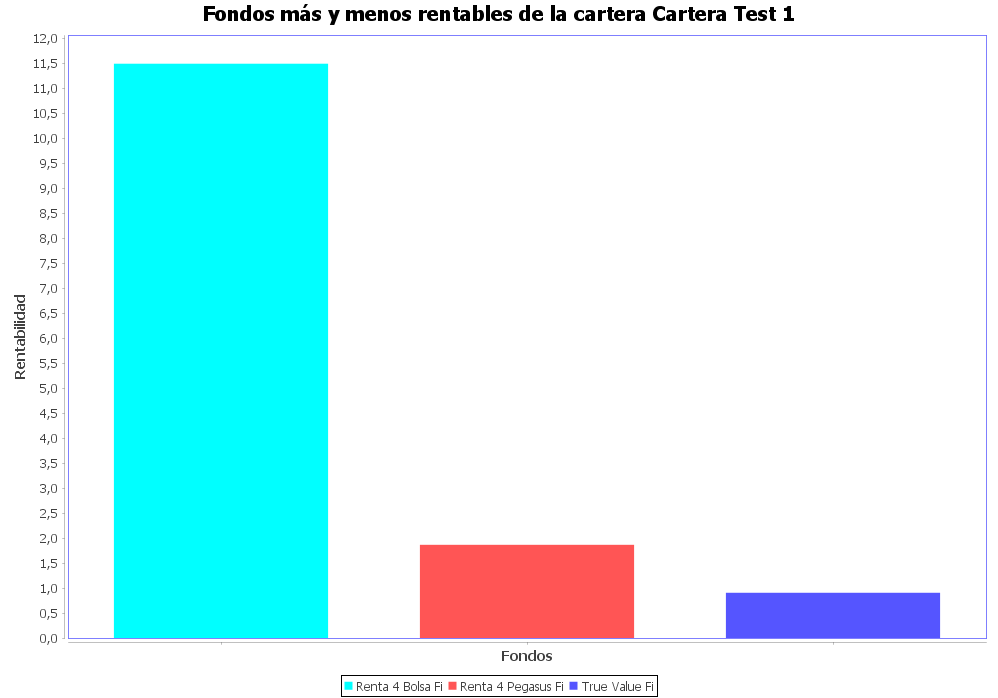
\includegraphics[width=\textwidth]{figuras/masrentables.PNG}
	\caption{Gráfica de los fondos más rentables de la cartera}
	\label{fig:masrentables}
	\end {figure}
	
Para calcular esta gráfica se tienen en cuenta la rentabilidad de todas las operaciones realizadas en la cartera, es decir, se calcula la rentabilidad entre el coste total de compras de participaciones y la remuneración de las ventas. Si las participaciones todavía no se han vendido entonces se calcula su valor a día de hoy y se suma al valor de venta.\\

En este caso nuestra cartera de prueba solo tiene tres fondos por lo que son, a la vez, los más y menos rentables de la cartera.\\

Es posible que alguno de los fondos menos rentables tengan una rentabilidad negativa. Si esto ocurre, simplemente la barra estará en sentido inverso.
	
\newpage
\subsubsection{Comparativa de inversión}

Esta gráfica tiene como objetivo mostrar una comparativa entre el valor de nuestras participaciones en la última operación realizada y el valor que poseen actualmente. Con esta información podemos ver rápidamente si el capital invertido en un determinado fondo ha crecido o menguado desde el último movimiento de participaciones.\\

Para visualizar los datos se utiliza una gráfica de barras, cada categoría es un fondo, la barra roja indica el valor de las participaciones en la última operación y la barra roja el valor actual.

	\begin{figure}[htbp]
	\centering
	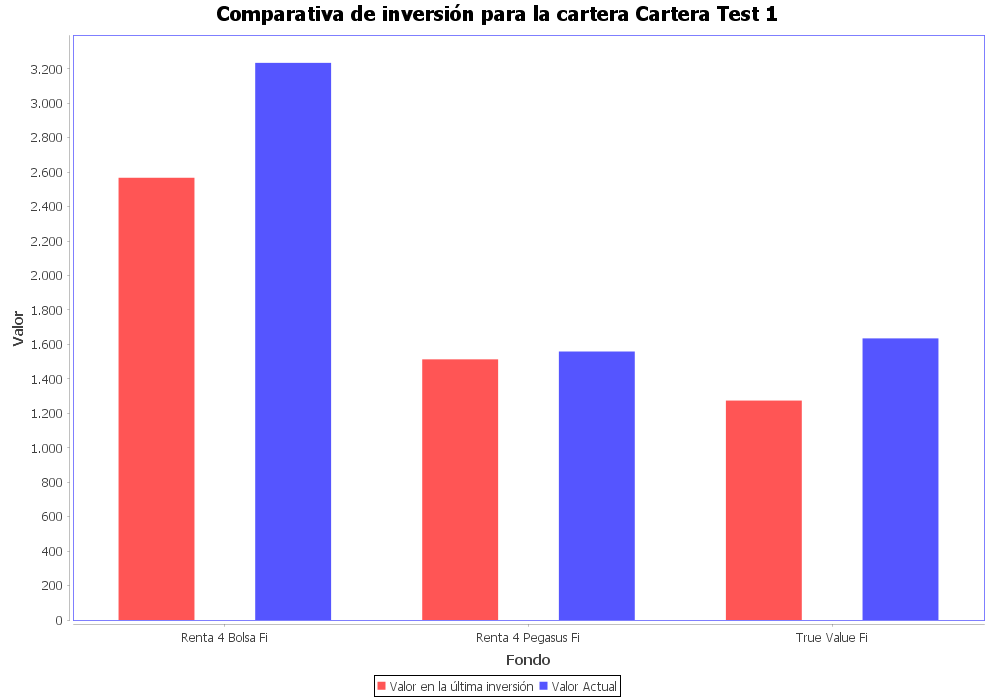
\includegraphics[width=\textwidth]{figuras/comparativa.PNG}
	\caption{Gráfica de la comparativa de inversión de la cartera}
	\label{fig:comparativa}
	\end {figure}

Para calcular esta gráfica simplemente deberemos obtener las participaciones finales de la última operación, su valor entonces y su valor actual.\\ 

Si un fondo de la cartera no tiene ninguna operación registrada o se han liquidado todas sus participaciones no aparecerá en esta gráfica.

\newpage

\subsubsection{Rentabilidad total de la cartera}

Esta gráfica tiene como objetivo mostrar la rentabilidad total de la cartera en un período de tiempo determinado. Con esta información podemos comprobar como evoluciona en el tiempo el conjunto de nuestras inversiones.\\

Para visualizar los datos se utiliza una gráfica de serie temporal.

	\begin{figure}[htbp]
	\centering
	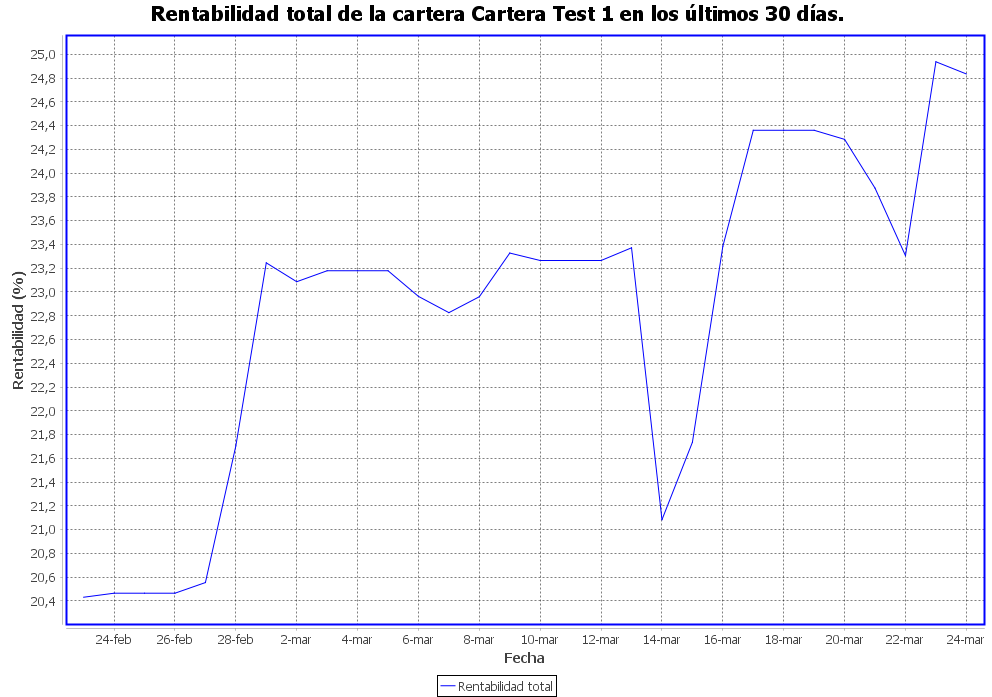
\includegraphics[width=\textwidth]{figuras/renttotal.PNG}
	\caption{Gráfica de la rentabilidad en conjunto de la cartera}
	\label{fig:renttotal}
	\end {figure}


Para calcular esta gráfica se calcula la rentabilidad de todos los fondos en función de las operaciones realizadas para cada día de la gráfica y luego se suman, obteniendo el total. Si para un día concreto tenemos participaciones de un fondo en la cartera, su precio se calcula multiplicándolas por el \gls{VL} más cercano.
\newpage

\subsection{Gráficas de fondos}

\subsubsection{Historial del Valor Liquidativo}

Esta gráfica tiene como objetivo mostrar un histórico de los \gls{VL}s del fondo seleccionado. Para ello se utiliza una gráfica de serie temporal. Este tipo de gráficas utilizan valores de tipo temporal en el eje de abscisas y valores de tipo double en el de ordenadas.\\

	\begin{figure}[htbp]
	\centering
	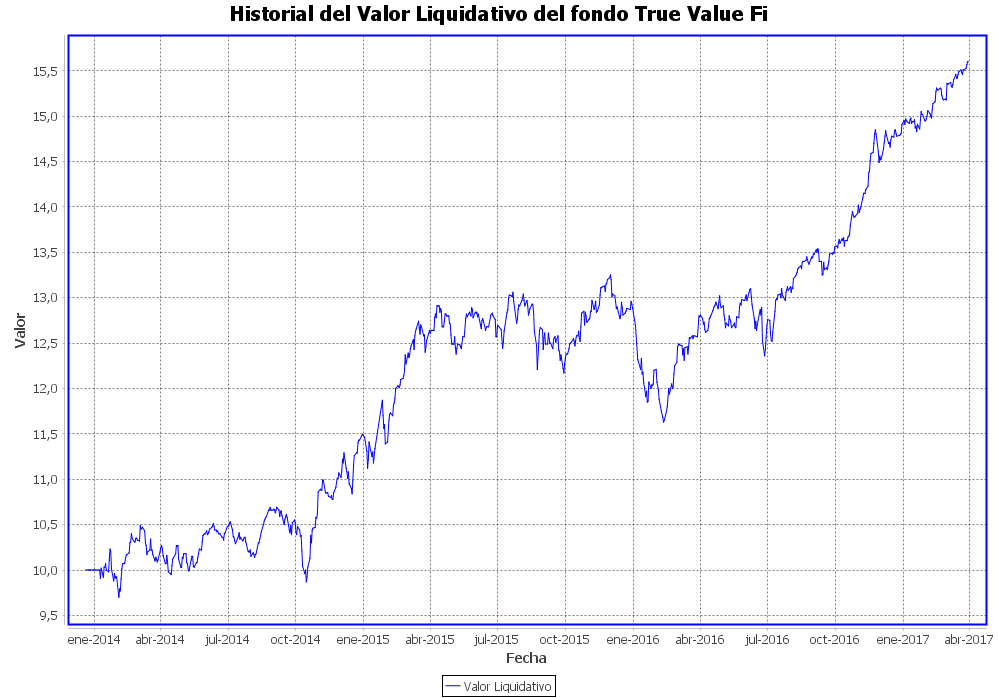
\includegraphics[width=\textwidth]{figuras/historial.PNG}
	\caption{Gráfica historial del Valor Liquidativo}
	\label{fig:historial}
	\end {figure}

El cálculo de esta gráfica es muy sencillo, basta con incluir en ella los \gls{VL}s del fondo en el período seleccionado.

\newpage

\subsubsection{Historial de rentabilidades}

Esta gráfica tiene como objetivo mostrar las rentabilidades históricas del fondo para los siguientes períodos de tiempo: último año fiscal, último semestre, último trimestre y último mes. Con esta información podemos ver como ha evolucionado el fondo en los últimos períodos de tiempo, y comprobar si ha tenido variaciones o si ha seguido una tendencia.\\

Para visualizar los datos se utiliza una gráfica de barras, cada categoría es un período de tiempo y la barra indica la rentabilidad en dicho período.

	\begin{figure}[htbp]
	\centering
	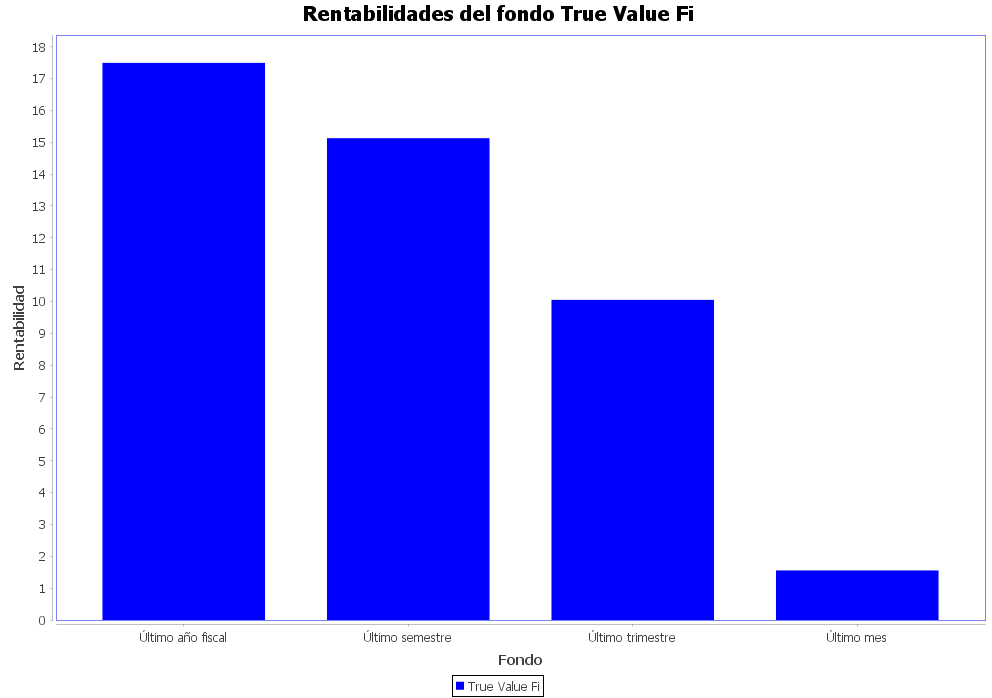
\includegraphics[width=\textwidth]{figuras/rentabilidades.PNG}
	\caption{Historial de rentabilidades}
	\label{fig:rentabilidades}
	\end {figure}

Para calcular esta gráfica obtenemos los \gls{VL} más próximos a las fechas de inicio y fin del período, si existe la suficiente distancia entre ellas calculamos sus rentabilidades, si por el contrario no hay suficientes días entre ellos obviamos ese período y lo indicamos en la descripción.

\newpage

\subsubsection{Rentabilidad esperada}

Esta gráfica tiene como objetivo mostrar un histórico de los \gls{VL}s del fondo seleccionado y los \gls{VL} esperados en función de la rentabilidad media diaria. Con esta información podemos ver una estimación de los \gls{VL}s del fondo y comparar los reales con los estimados.\\

Para visualizar los datos se utiliza una gráfica de serie temporal.

	\begin{figure}[htbp]
	\centering
	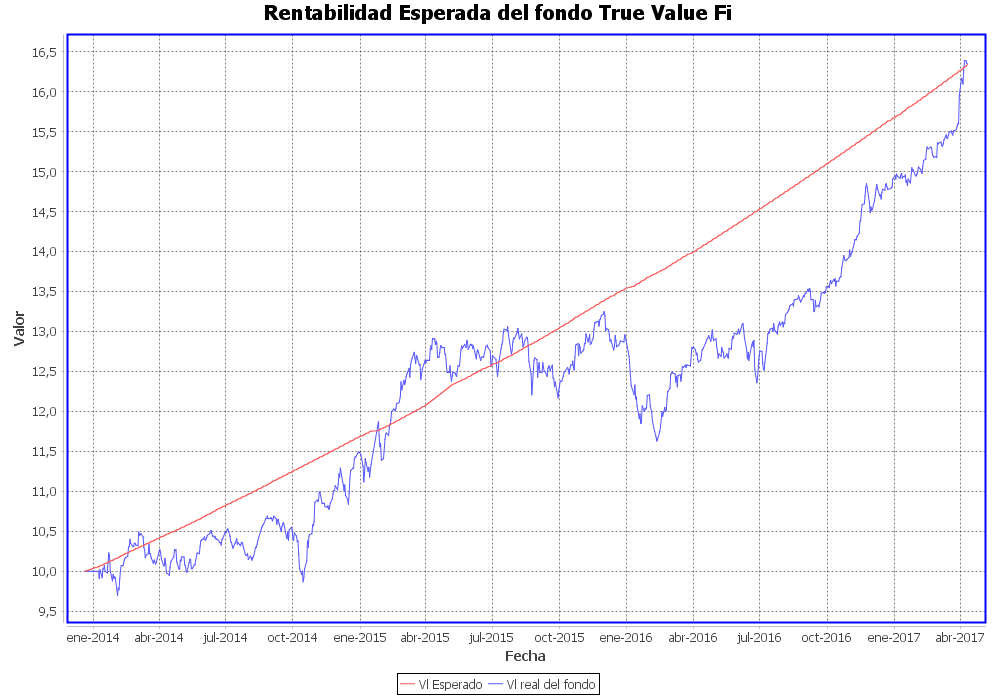
\includegraphics[width=\textwidth]{figuras/esperada.PNG}
	\caption{Rentabilidad esperada}
	\label{fig:esperada}
	\end {figure}

Para calcular esta gráfica se utiliza la rentabilidad media diaria $r$. Este valor nos indica la variación diaria teniendo en cuenta todos los datos disponibles del fondo. Para calcularla se utilizan los valores liquidativos más antiguo y más reciente, esto es, $\text{VL}_I$ y $\text{VL}_F$, respectivamente.

\begin{equation}
r=\left(\frac{\text{VL}_F}{\text{VL}_I}\right)^{1/d}-1
\end{equation} 
Donde $d$ es el número de días transcurridos entre los valores liquidativos inicial y final.\\

Una vez calculado r se añade el primer valor a la gráfica, el resto se calculan de la siguiente manera.

\begin{equation}
e_i= e_{i-1} \left(1 + r\right), \quad\text{para }i>1
\end{equation} 



\newpage

\subsubsection{Medias Móviles}

Esta gráfica tiene como objetivo mostrar un histórico de los \gls{VL}s del fondo seleccionado y su media móvil a un determinado intervalo de tiempo. Una de las grandes ventajas de usar medias móviles es que se mueven en la dirección de la tendencia, lo que permite que avancen los beneficios y se frenen las pérdidas. Pero hay que tener en cuenta que su uso es para seguir la pista de la tendencia, la media no anticipa nada.


	\begin{figure}[htbp]
	\centering
	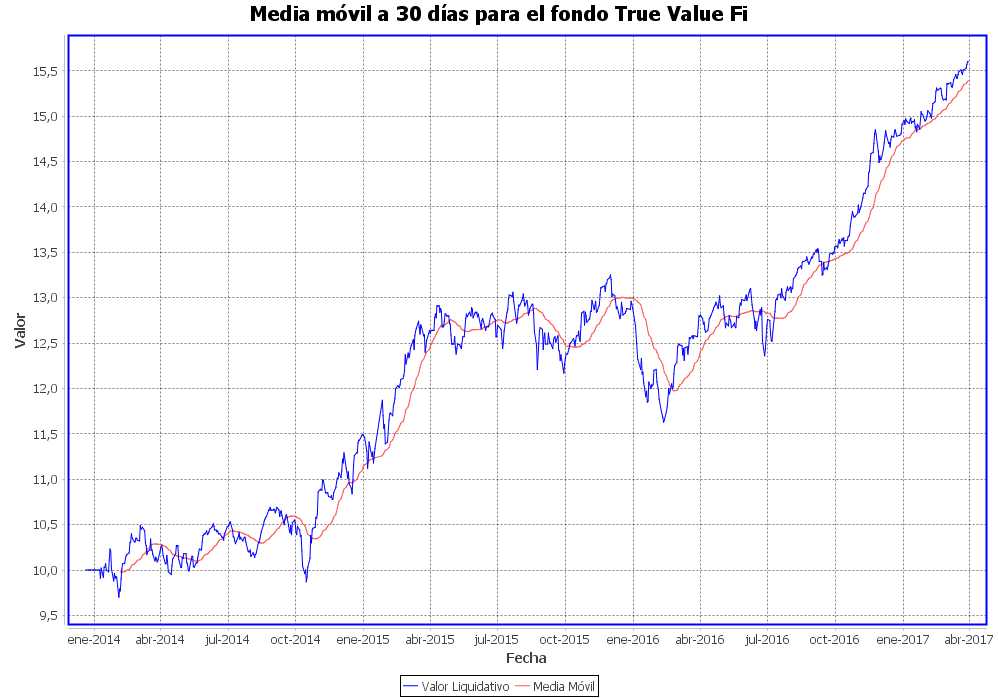
\includegraphics[width=\textwidth]{figuras/media.PNG}
	\caption{Media Móvil}
	\label{fig:media}
	\end {figure}
	
	Para calcular esta gráfica supongamos el fondo tiene los siguientes valores liquidativos $\text{VL}_1,\text{VL}_2,\ldots,\text{VL}_d$ para los días $1,2,\ldots,d$, y que queremos calcular la media móvil para $m$ días. En ese caso, tendremos una secuencia de $d-m+1$ valores $y_m,y_{m+1},\ldots,y_d$. Los primeros $m-1$ valores de la secuencia $y$ se pueden poner a $0$. El resto de valores se calculan de la siguiente manera:
	
	\begin{equation}
	y_j=\frac{1}{m}\left(\sum_{i=j-m+1}^{j}\text{VL}_i\right)
	\end{equation}
	De forma más eficiente, suponiendo que se ha calculado el primer valor de la serie, $y_m$, tenemos:
	
	\begin{equation}
	y_{j}=\frac{1}{m}\left(m\cdot y_{j-1}+\text{VL}_j-\text{VL}_{j-m}\right),\quad\text{para }j>m
	\end{equation}

\newpage

\section{Cuarta iteración: Ejecución de tareas en segundo plano}

Esta cuarta iteración tiene como objetivo implementar la ejecución en segundo plano de las tareas que requieren un cierto tiempo de procesamiento.\\

Para ello, Swing nos proporciona \textbf{SwingWorker}, una clase abstracta para realizar interacciones con la \gls{GUI} en un thread en segundo plano.

\subsection{SwingWorker}

Cuando construimos una aplicación multi-thread utilizando Swing, debemos tener en cuenta dos restricciones:

\begin{itemize}
	\item Las tareas que consumen tiempo no deberían correr en el \gls{EDT}, pues la aplicación se quedaría congelada.
	\item Los componentes de swing únicamente deberían ser accesibles en el \gls{EDT}.
\end{itemize}

Estas restricciones significan que una \gls{GUI} con tareas que requieren un tiempo de cómputo grande necesitan por lo menos dos threads: uno para realizar las tareas largas y otro, el \gls{EDT}, para las actividades relacionadas con los componentes de la interfaz.\\

Podríamos realizar esta tarea a mano, usando la clase Thread para crear un hilo cada vez que realizemos una tarea que requiera tiempo, pero desde java 6 tenemos SwingWorker.\\

SwingWorker está diseñado para situaciones en las que se necesita tener una tarea larga corriendo en segundo plano y proveer actualizaciones a la \gls{GUI} acerca de si ha terminado, o sigue en proceso.\\

La clase SwingWorker es una clase abstracta en la que debemos definir dos tipos de datos: Class SwingWorker$<$T,V$>$. T representa el tipo de objeto devuelto cuando el worker termina la tarea, mientras que V es el tipo de información que que usara el worker para informar de su progreso.\\

Todas las subclases de SwingWorker deben implementar el método doInBackground(), donde se implementará la tarea en segundo plano, y el método done(), en el que se muestra el resultado de la operación en pantalla. SwingWorker se encargará de que ambos métodos se ejecuten en los threads adecuados.\\

 Cuando creamos un SwingWorker debemos pasar como parámetros aquellos elementos que queramos modificar cuando se complete la operación, y modificarlos unicamente en el método done(). En este último método también se capturan las excepciones ocurridas durante el transcurso de doInBackground().\\
 
 Para ejecutar un worker, basta con llamar a su método execute(). Esta llamada crea el nuevo thread y devuelve el control inmediatamente.
 
 \newpage
 
Si queremos informar del progreso de la operación, en el método doInBackground() podemos llamar a setProgress() (un método que admite un entero entre 0 y 100) o publish() (que utilizara el tipo de dato que hayamos definido en V). Ambos métodos notifican a los PropertyChangeListener con un evento denominado progress, que podemos capturar y utilizar para mostrar al usuario o actualizar una barra de progreso.\\


Existen tres threads involucrados en el ciclo de vida de un SwingWorker:

\begin{itemize}
	\item El thread actual: Es donde se llama el método execute(). Esto programa a SwingWorker para la ejecución en segundo plano de la tarea en lo que se denomina worker thread, y vuelve al hilo actual. Podemos esperar a que se complete dicha operación con el método get(), lo que bloquearía la interfaz.
	\item El worker thread: el método doInBackground() se llama en este thread. En el se llevan a cabo las tareas necesarias y se notifica a los PropertyChangeListeners acerca del estado de la tarea.
	\item El \gls{EDT}: todas las actividades relacionadas con Swing ocurren en este thread. SwingWorker invoca el método done() y notifica a cualquier PropertyChangeListener en este hilo.
\end{itemize}

Normalmente el thread actual se corresponde con el \gls{EDT}.\\

Antes de que se ejecute el metodo doInBackground, SwingWorker notifica a todos los PropertyChangeListeners acerca del cambio de estado a StateValue.STARTED. Una vez termina doInBackground y se ejecuta el método done, se notifica que el estado pasa a StateValue.DONE.\\

En última instancia hemos de tener en cuenta que:

\begin{itemize}
	\item Si por alguna razón queremos cancelar un worker en ejecución, es necesario llamar al método cancel(true), que interrumpe la operación.
	\item SwingWorker está diseñado para ser ejecutado una única vez. Ejecutar el mismo worker una segunda vez no tendrá ningún efecto.
\end{itemize}


\newpage

\subsection{Implementación de SwingWorker}

Existen tres tareas en nuestra aplicación que pueden tardar un tiempo suficiente en realizarse como para que el usuario perciba que la interfaz se ha quedado bloqueada: Importar un fondo o los \gls{VL}s de un fondo, crear las gráficas y actualizar el árbol de carteras.

\subsubsection{ChartWorker}

Hasta ahora la clase encargada de crear las gráficas era \textit{``ChartMaker"}, una clase a la que le pasábamos los parámetros necesarios y nos devolvía un objeto de tipo \textbf{Chart}, el cual contenía la gráfica y una descripción.\\

Para poder ejecutar las gráficas en segundo plano y tener información acerca de su progreso, ha sido necesario modificar esta clase de tal manera que herede de SwingWorker, de esta manera podemos redefinir los métodos doInBackground() y done(). Para indicar que esta clase se ejecutará en un worker thread se ha cambiado su nombre a \textit{``ChartWorker"}. \\

Como hemos definido en el punto anterior, la tarea que se realizará en segundo plano es la contenida en el método doInBackground(), con el objetivo de evitar el tener que crear una clase worker para cada gráfica, se ha creado un constructor genérico donde se proporcionan los elementos de la interfaz que se actualizan cuando la gráfica está terminada (cuando se llama al método done()).\\

Para seleccionar la gráfica que queremos crear debemos llamar a un método de la clase y pasarle los valores necesarios para crear esa gráfica en concreto. Por ejemplo, para crear la gráfica de distribución del capital primero deberemos llamar a setPortfolioDistributionChart() donde indicamos la cartera de la cual queremos obtener la gráfica y a continuación al método execute().\\

Cuando la tarea termina, el resultado obtenido es exactamente el mismo que antes, un objeto Chart con la gráfica y la descripción. Sin embargo, el panel y el cuadro de la descripción se actualizan directamente en el método done(), en lugar de en la clase principal, para asegurarnos que los componentes siempre se actualizan en el \gls{EDT} una vez ha terminado la operación. Si por cualquier motivo falla la ejecución de la tarea, en el método done() capturamos la excepción \textit{ExecutionException} y reseteamos el panel de las gráficas.\\

Normalmente en un equipo medio y para fondos normales (el fondo más extenso que se ha utilizado cuenta con alrededor de 7000 valores desde 1993) todas las gráficas excepto la de la rentabilidad total de la cartera no tardan más de medio segundo en crearse. Esta última en cambio tarda alrededor de unos cinco segundos porque tiene que calcular un gran número de operaciones y  será la única que reporte su progreso mediante el método setProgress().\\


\newpage

Para poder mostrar el progreso en la barra de la ventana principal es necesario añadir un PropertyChangeListener que reaccione ante el evento progress cuando creemos el worker. De esta manera la barra se actualizará conforme avance la tarea indicando al usuario el progreso.\\


Durante la realización de la gráfica es posible que el usuario cambie a otra o realice otra operación sin esperar a que esta termine. Si esto sucede, el usuario podría estar viendo ya otra gráfica y de repente se le actualizaría el panel con la rentabilidad total de la cartera. Para evitar esta situación, cada vez que se seleccione otra gráfica mientras se está calculando la rentabilidad, cancelaremos la operación pendiente mediante el método cancel(true).


\subsubsection{NodesWorker}

La segunda tarea que queremos ejecutar en segundo plano es la de actualizar el árbol de carteras.\\

Esta operación estaba realizada por la función createNodes(), que solicitaba los datos de carteras y fondos a la base de datos y construía el árbol. Para ejecutar esta tarea en un worker thread, se ha creado una nueva clase denominada NodesWorker.\\

El método doInBackground() realiza la misma función que createNodes(). Al actualizar el modelo del árbol con los datos nuevos este se contrae por defecto y el último elemento seleccionado se des selecciona. Para evitar esto, en el método done() se ha establecido un comportamiento para el último elemento:

\begin{itemize}
	\item Si el nodo aún existe, se selecciona de nuevo y se expande el recorrido hasta él.
	\item Si el nodo ya no existe, se selecciona su nodo padre.
\end{itemize} 

La operación informa periódicamente del progreso mediante el método setProgress(), por lo que, al igual que en el caso anterior, es necesario añadir un PropertyChangeListener que reaccione ante el evento progress cuando creemos el worker, pero en este caso será la barra inferior de progreso la que se actualice a medida que se actualiza el árbol.

\subsubsection{ImportFundWorker}

Por último, nos queda la tarea de importar fondos o \gls{VL}s.\\

El funcionamiento de este worker es muy similar al de las gráficas. De nuevo se ha creado un constructor genérico donde se proporcionan los elementos de la interfaz que se actualizan cuando la operación está terminada. A mayores se le proporciona una instancia de un NodesWorker, de esta manera es posible actualizar el modelo una vez se termine de importar.\\

Para seleccionar la operación que queremos utilizar debemos llamar a un método de la clase y pasarle los valores necesarios para realizar esa operación en concreto. Por ejemplo, para importar los \gls{VL}s de un fondo, debemos proporcionar el fondo en el que se importarán y el formato de la fecha del fichero.\\

\newpage

Cuando importamos los \gls{VL}s de un fondo comprobamos si existe un valor para el día de cada uno en la base de datos. Si existe, se actualiza el que tenemos, sino, se añade el nuevo. En este caso, como en los anteriores, se utiliza setProgress() para indicar el progreso de la operación.\\

Cuando importamos un fondo, el servicio del modelo nos devuelve el fondo contenido en el fichero junto con sus \gls{VL}s asociados. En este caso no es posible conocer el progreso de la operación en un momento determinado, por lo que utilizamos el método setIndeterminate() de la barra de progreso para indicar que se está realizando una operación.\\

Mientras se está importando un fondo o sus \gls{VL}s, se bloquean los botones de importar fondo e importar \gls{VL}s.
\newpage

\appendix
\chapter{Manual de usuario}\label{aped.A}


\cleardoublepage

\newpage

\begin{thebibliography}{10}
	
	\bibitem[ Bou Ysas Silvia]{}
	\newblock {\textit{Medidas de Performance Para Carteras de Fondos de Inversión}.
		\\Ewe Editorial Acad MIA Espa Ola , 2012.}
	
	\bibitem[CNMV]{}
	\newblock {\textit{Comisión Nacional del Mercado de Valores}.}
	\newline
	\href{https://www.cnmv.es/}{https://www.cnmv.es/}
	
	\bibitem[Rankia]{}
	\newblock {\textit{Todo lo que hay que saber de Fondos de inversión en un único artículo}.}
	\newline
	\href{http://www.rankia.com/blog/fondos-inversion/3208096-todo-que-hay-saber-fondos-inversion-unico-articulo}{http://www.rankia.com/blog/fondos-inversion/3208096-todo-que-hay-saber-fondos-inversion-unico-articulo}
	
	\bibitem[Rankia]{}
	\newblock {\textit{¿Qué es un fondo de inversión y cómo funciona?}.}
	\newline
	\href{http://www.rankia.com/blog/fondos-inversion/952310-que-fondo-inversion-como-funciona}{http://www.rankia.com/blog/fondos-inversion/952310-que-fondo-inversion-como-funciona}
	
	\bibitem[Rankia]{}
	\newblock {\textit{Índice de referencia del fondo}.}
	\newline
	\href{https://www.rankia.com/blog/fondos-inversion-que-es/1137719-indice-referencia-fondo}{https://www.rankia.com/blog/fondos-inversion-que-es/1137719-indice-referencia-fondo}
	
	\bibitem[Rankia]{}
	\newblock {\textit{Máximo drawdown}.}
	\newline
	\href{https://www.rankia.com/blog/fondos-inversion-que-es/1137747-maximo-drawdown}{https://www.rankia.com/blog/fondos-inversion-que-es/1137747-maximo-drawdown}
	
	\bibitem[Funds Peopel]{}
	\newblock {\textit{La importancia de la ratio de Sharpe a la hora de seleccionar fondos}.}
	\newline
	\href{http://es.fundspeople.com/news/la-importancia-del-ratio-de-sharpe-a-la-hora-de-seleccionar-fondos}{http://es.fundspeople.com/news/la-importancia-del-ratio-de-sharpe-a-la-hora-de-seleccionar-fondos}
	
	\bibitem[Economipedia]{}
	\newblock {\textit{Alfa de Jensen}.}
	\newline
	\href{http://economipedia.com/definiciones/alfa-de-jensen.html}{http://economipedia.com/definiciones/alfa-de-jensen.html}
	
	\bibitem[Economipedia]{}
	\newblock {\textit{Beta de un activo financiero}.}
	\newline
	\href{http://economipedia.com/definiciones/beta-de-un-activo-financiero.html}{http://economipedia.com/definiciones/beta-de-un-activo-financiero.html}
	
	\bibitem[Wikipedia]{}
	\newblock {\textit{Proceso Unificado de Desarrollo Software}.}
	\newline
	\href{https://es.wikipedia.org/wiki/Proceso\_unificado}{https://es.wikipedia.org/wiki/Proceso\_unificado}
	
	\bibitem[Wikipedia]{}
	\newblock {\textit{Model–view–presenter}.}
	\newline
	\href{https://en.wikipedia.org/wiki/Model–view–presenter}{https://en.wikipedia.org/wiki/Model–view–presenter}
	
	\bibitem[Jboss]{}
	\newblock {\textit{Hibernate}.}
	\newline
	\href{http://docs.jboss.org/hibernate/orm/3.5/reference/es-ES/html/}{http://docs.jboss.org/hibernate/orm/3.5/reference/es-ES/html/}
	
	\newpage
	
	\bibitem[Mkyong]{}
	\newblock {\textit{Hibernate, Many-to-Many annotation}.}
	\newline
	\href{https://www.mkyong.com/hibernate/hibernate-many-to-many-relationship-example-annotation/}{https://www.mkyong.com/hibernate/hibernate-many-to-many-relationship-example-annotation/}
	
	
	
	\bibitem[Vladmihalcea]{}
	\newblock {\textit{The best way to map a Composite Primary Key with JPA and Hibernate}.}
	\newline
	\href{https://vladmihalcea.com/2016/08/01/the-best-way-to-map-a-composite-primary-key-with-jpa-and-hibernate/}{https://vladmihalcea.com/2016/08/01/the-best-way-to-map-a-composite-primary-key-with-jpa-and-hibernate/}
	
	\bibitem[Oracle]{}
	\newblock {\textit{Using Swing Components}.}
	\newline
	\href{http://docs.oracle.com/javase/tutorial/uiswing/components/index.html}{http://docs.oracle.com/javase/tutorial/uiswing/components/index.html}
	
	\bibitem[Oracle]{}
	\newblock {\textit{Writing Event Listeners}.}
	\newline
	\href{http://docs.oracle.com/javase/tutorial/uiswing/events/index.html}{http://docs.oracle.com/javase/tutorial/uiswing/events/index.html}
	
	\bibitem[CodeJava]{}
	\newblock {\textit{How to use JDatePicker to display calendar component}.}
	\newline
	\href{http://www.codejava.net/java-se/swing/how-to-use-jdatepicker-to-display-calendar-component}{http://www.codejava.net/java-se/swing/how-to-use-jdatepicker-to-display-calendar-component}
	
	\bibitem[Java Creed]{}
	\newblock {\textit{Swing Worker}.}
	\newline
	\href{http://www.javacreed.com/swing-worker-example/}{http://www.javacreed.com/swing-worker-example/}
	
	\bibitem[Java Code Geeks]{}
	\newblock {\textit{Multi-threading in Java Swing with SwingWorker}.}
	\newline
	\href{https://www.javacodegeeks.com/2012/12/multi-threading-in-java-swing-with-swingworker.html}{https://www.javacodegeeks.com/2012/12/multi-threading-in-java-swing-with-swingworker.html}
	
	\bibitem[jfree]{}
	\newblock {\textit{JFreeChart - Documentation}.}
	\newline
	\href{http://www.jfree.org/jfreechart/api/javadoc/index.html}{http://www.jfree.org/jfreechart/api/javadoc/index.html}
	
	\bibitem[Tutorials Point]{}
	\newblock {\textit{JFreeChart Tutorial}.}
	\newline
	\href{https://www.tutorialspoint.com/jfreechart/}{https://www.tutorialspoint.com/jfreechart/}
	
	\bibitem[jexcelapi]{}
	\newblock {\textit{JexcelApi - Documentation}.}
	\newline
	\href{http://jexcelapi.sourceforge.net/resources/javadocs/}{http://jexcelapi.sourceforge.net/resources/javadocs/}
	
	
	\bibitem[TeamDev]{}
	\newblock {\textit{JexcelApi - JExcel Programmer's Guide}.}
	\newline
	\href{https://www.teamdev.com/downloads/jexcel/docs/JExcel-PGuide.html}{https://www.teamdev.com/downloads/jexcel/docs/JExcel-PGuide.html}
	
	
\end{thebibliography}
\newpage
\setglossarystyle{tree}
\printglossary[type=\acronymtype]

\end{document}